\documentclass[a4paper,12pt,twoside,final]{scrbook}
\usepackage[utf8]{inputenc}
\usepackage[spanish,es-nodecimaldot]{babel} % International, rec. by RAE: http://www.tex-tipografia.com/marca_decimal.html

\usepackage{booktabs}
\usepackage[hidelinks]{hyperref}

\usepackage{tgpagella} % text only
\usepackage{mathpazo}  % math & text

\usepackage{tabularx}
\usepackage{placeins}

\usepackage{setspace}
\spacing{1.2}

% COLOR
\usepackage[usenames,dvipsnames,svgnames,table]{xcolor}
% Colores para estilo Proyecto Docente (tonos naranjas)
\definecolor{lightback}{HTML}{F4E0BF}
     \definecolor{back}{HTML}{F3C591}
\definecolor{lightline}{HTML}{FCAF5F}
     \definecolor{line}{HTML}{ED7900}
% Colores para portada
\definecolor{epsc:oscuro}{HTML}{280091}
 \definecolor{epsc:medio}{HTML}{4C5CC5}
 \definecolor{epsc:claro}{HTML}{3FCFD5}
 \definecolor{epsc:verde}{HTML}{00B299}

\usepackage{verbatim}
\usepackage{tikz} % used in cover to place images
\usetikzlibrary{babel,arrows,positioning,fit}
\usepackage[simplified]{pgf-umlcd}
\usepackage{pgf-umlsd}

\usepackage{datetime} % allow formal date format
% "Month, YEAR" date format, in spanish with the month uppercased not interfering other dates
\newcommand\Monthname[1][EMPTY]{
  \ifnum1=#1Enero\else
  \ifnum2=#1Febrero\else
  \ifnum3=#1Marzo\else
  \ifnum4=#1Abril\else
  \ifnum5=#1Mayo\else
  \ifnum6=#1Junio\else
  \ifnum7=#1Julio\else
  \ifnum8=#1Agosto\else
  \ifnum9=#1Septiembre\else
  \ifnum10=#1Octubre\else
  \ifnum11=#1Noviembre\else
  \ifnum12=#1Diciembre\else
  \fi\fi\fi\fi\fi\fi\fi\fi\fi\fi\fi\fi
}
\newdateformat{monthyeardate}{%
  \Monthname[\THEMONTH], \THEYEAR}


% FONTs
\usepackage[T1]{fontenc}
\usepackage{textcomp}           % Needed for new symbols like € ?

\usepackage[scaled]{berasans} % Font for the cover similar to Vera 33
%\renewcommand*\familydefault{\sfdefault}  %% To use as the base font of the document is to be sans serif


% PAGE STYLE
\usepackage[twoside,bindingoffset=0mm,headheight=16pt,margin=25mm]{geometry} %,verbose,showframe
%\usepackage{fancyhdr} % Encabezados
%\pagestyle{fancy}
% XXX Evitar el binding en la portada pero no en el resto del documento

% TABLES AND FIGURES
\usepackage{graphicx}
\graphicspath{ {img/} }

% SUBRALLADOS
\usepackage[normalem]{ulem}

\usepackage{longtable}



\begin{document}
%\frontmatter

%------------- Cover --------------
\thispagestyle{empty}

% Backgroud images
\begin{tikzpicture}[remember picture, overlay]
  % Top
  \node [anchor=north east, inner sep=0pt]  at (current page.north east)
     {
\includegraphics[height=6cm]{topRightCorner.pdf}};
  % Bottom
  \node [anchor=south west, inner sep=0pt]  at (current page.south west)
     {
\includegraphics[height=6cm]{bottomLeftCorner.pdf}};
  \node (uco) [anchor=south east, inner sep=0pt, xshift=-10mm, yshift=10mm]  at (current page.south east)
        {
\includegraphics[height=2cm]{uco_debajo.pdf}};
  \node [anchor=south east, inner sep=0pt, xshift=-10mm]  at (uco.south west)
% Uncomment the chosen logo and comment the others:
        {
\includegraphics[height=2cm]{emblema-ing-informatica.pdf}};
%        {\includegraphics[height=2cm]{emblema-ing-industrial.pdf}};
%        {\includegraphics[height=2cm]{emblema-ing-tec-industrial.pdf}};
\end{tikzpicture}


\begin{center}
\fontfamily{\sfdefault}\selectfont
\vspace*{2cm}

\vfill
\vfill

\includegraphics[width=12.5cm]{LogotipoEPSC.pdf}
\vfill
\vfill

\large\textbf{\color{epsc:medio}
  TRABAJO FIN DE GRADO EN INGENIERÍA INFORMÁTICA
}
\vfill

\Huge\textbf{\color{epsc:oscuro}
  Plataforma web de gestión de comunicados
}
\vfill
\vfill

\Large\textbf{\color{epsc:verde}
  MEMORIA TÉCNICA
}
\vfill
\vfill

\large{\color{epsc:oscuro}Autor}\\
\textbf{\color{epsc:medio}{ Eduardo Arroyo Ramírez }}
\vfill

\large{\color{epsc:oscuro} Director }\\
\textbf{\color{epsc:medio} Domingo Ortiz Boyer}
\vfill



\textbf{\color{epsc:verde} \monthyeardate\today}
\vfill
\vfill
\vspace{2.7cm}
\end{center}

%-------------------------------------------------------------------------------
\clearpage

\thispagestyle{empty}
\pagecolor{white}

\cleardoublepage
%-------------------------------------------------------------------------------
\frontmatter
\tableofcontents
\listoffigures
\listoftables

\cleardoublepage
\mainmatter
\part{Presentación}
\chapter{Introducción}
Contexto sobre el origen de este proyecto: empresa pequeña queriendo entrar en el mercado de aplicaciones móviles de bajo coste y escalables.
\chapter{Definición del problema}

\section{La comunicación corporativa}
La \emph{Comunicación Corporativa} se define como <<la totalidad de los recursos de comunicación de los que dispone una organización para llegar efectivamente a sus públicos>> \cite{riel_2001}. Dentro de este concepto, se distingue entre la \emph{Comunicación Corporativa Interna} y la \emph{Comunicación Corporativa Externa} siendo la primera <<todo lo relativo a la conexión requerida entre los miembros de una determinada estructura para acometer una metas comunes>> y la segunda, <<la vinculación de la organización con el entorno en el que desarrolla sus actividades, con el fin de alcanzar un determinado nivel de rentabilidad económica y social>> \cite{castro_2007}. Desde el ámbito empresarial y administrativo se da cada vez mayor importancia a la comunicación ya que ésta juega un papel fundamental en la consecución de sus objetivos.

Este tipo de comunicación ha encontrado en Internet uno de sus canales principales y tanto empresas como instituciones ejercen hoy en día su presencia online a través de webs, blogs, redes sociales o incluso sus propias aplicaciones para móviles, que han proliferado enormemente durante los últimos años \cite{playstore} \cite{appstore}. Todas estas herramientas permiten no sólo la publicación de comunicados sino también la planificación temporal, seguimiento y medida del impacto.

\section{Aplicaciones para móviles}
Aunque las redes sociales son uno de los medios preferidos por las empresas \cite{linkedin} y administraciones \cite{grande2015casos} como canal de comunicación debido a la gran acogida que tienen entre la población, las aplicaciones móviles son una alternativa muy a tener en cuenta ya que cubren la frecuente necesidad de incluir otros servicios específicos de la organización como por ejemplo:
\begin{itemize}
    \item Sistema de reservas (mesas en un restaurante, salas en un gimnasio\dots).
    \item Encuestas (toma de decisiones en una comunidad de vecinos, sondeo de la clientela de un bar para organizar un concierto en directo\dots)
    \item Sistema de geolocalización en tiempo real de un desfile (¿por dónde está pasando ahora mismo la cabalgata de reyes?).
\end{itemize}
Además, las aplicaciones salvan algunos de los inconvenientes de las redes sociales como la cesión de datos, la alta exposición a la crítica o la obligación de adaptarse al diseño y las reglas de negocio impuestas por un tercero.
También es necesario mencionar el enorme desarrollo que ha tenido el acceso a internet desde dispositivos móviles en los últimos años, como se puede observar en la figura \ref{fig:acceso-internet-tipo-dispositivo} \cite{dispositivos_internet_2019}.

\begin{figure}[ht]
    \centering
    % https://www.ontsi.red.es/es/indicadores/Hogares-y-ciudadanos/Internet/Dispositivos-de-acceso-Internet
    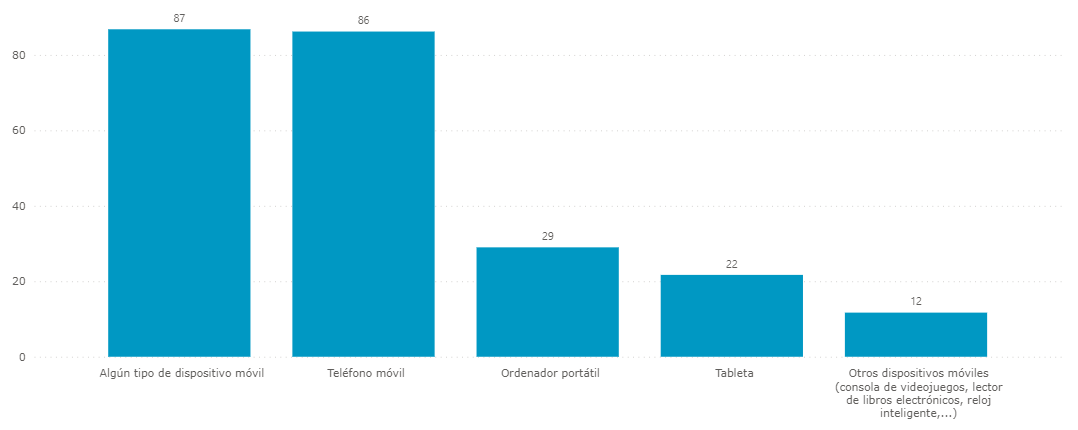
\includegraphics[scale=.5]{AccesoAInternetPorTipoDispositivo2019.png}
    \caption{Personas que han usado Internet en los últimos tres meses por tipo de dispositivo utilizado }
    \label{fig:acceso-internet-tipo-dispositivo}
\end{figure}
\chapter{Objetivos}

El objetivo general de este trabajo es la creación de una plataforma software que permita ofrecer en poco tiempo y a coste reducido aplicaciones móviles personalizadas asociadas a un gestor de contenidos que permita a diferentes organizaciones realizar la gestión básica y seguimiento del impacto de sus comunicaciones corporativas.

Para la consecución de dichos objetivos, se establecen los siguientes objetivos específicos:

\section{Plataforma de publicación y seguimiento de comunicados}
Es necesario dotar al sistema de una herramienta que permita a los editores preparar, publicar, programar y  consultar el impacto de los comunicados. Para ello se desarrollará una aplicación web que cubrirá las siguientes necesidades según el tipo de usuario:
\begin{itemize}
    \item Lectores (acceso público)
    \begin{itemize}
        \item Consulta pública de comunicados de la organización.
        \item Consulta de otros datos de interés de la organización (teléfonos, direcciones, etc.).
    \end{itemize}
    \item Editores (acceso restringido por organización)
    \begin{itemize}
        \item Administración de comunicados.
        \item Consulta de métricas de impacto de comunicaciones.
        \item Administración de tipos de registro independientes como categorías de comunicaciones, teléfonos, direcciones, etc. de la organización.
    \end{itemize}
    \item Administradores (responsables del mantenimiento del servicio)
    \begin{itemize}
        \item Administración de organizaciones.
        \item Administración de funcionalidades personalizadas disponibles para cada organización.
        \item Administración de usuarios.
        \item Configuración del servicio.
    \end{itemize}
\end{itemize}

\section{Servicio WEB de consulta de comunicados}
Para brindar acceso a los comunicados a través de aplicaciones propias o de terceros, es necesario dotar a la plataforma de un servicio WEB con una API pública que ofrezca los métodos necesarios para realizar dicha labor.
\begin{itemize}
    \item Lectores (acceso público)
    \begin{itemize}
        \item Consulta pública de comunicados de la organización.
        \item Consulta de otros datos de interés de la organización (teléfonos, direcciones, etc.).
    \end{itemize} 
\end{itemize}

\section{Aplicación móvil tipo}
Se desarrollará un prototipo aplicación móvil que consumirá el servicio web de la plataforma mediante solicitudes HTTP. Este prototipo será precursor de las aplicaciones finales que se desarrollen en el futuro para clientes y al mismo tiempo permitirá demostrar las capacidades del sistema.
\chapter{Antecedentes}

\section{Introducción}
En este apartado se analizan brevemente herramientas existentes que, o bien son similares o bien tienen objetivos parecidos a \emph{PushNews}. Se han seleccionado herramientas de comunicación corporativa como boletines informativos o webs corporativas y también de marketing digital como las que se utilizan para gestionar redes sociales.

\section{Newsletter o boletín informativo}
Una newsletter es una publicación digital periódica que se distribuye a través de correo electrónico. Generalmente recopila los artículos o comunicados publicados desde el último envío. Los receptores de una newsletter son personas que han mostrado previamente interés en el tema y se han suscrito a la publicación para recibirla en su bandeja de correo electrónico. La newsletter sigue siendo a día de hoy una herramienta muy importante en la comunicación corporativa por varias razones según Wikipedia \cite{wiki_boletininformativo}:
\begin{enumerate}
    \item Es un canal que, bien usado, permite construir una relación de confianza con el suscriptor que puede ser la base de futuras ventas.
    \item La calidad como lectores/clientes de las personas suscritas suele ser superior a los lectores esporádicos que encuentran llegan al sitio web, por ejemplo, a través de los buscadores.
    \item Porque es un activo que el autor de la lista tiene bajo su total control, a diferencia, por ejemplo, de los seguidores en redes sociales como Facebook o Twitter.
\end{enumerate}

Por otra parte, las newletters presentan algunas desventajas como las siguientes:
\begin{enumerate}
    \item Puede ser difícil conseguir que el que el usuario dé su consentimiento para recibir la newsletter.
    \item A menudo se considera spam.
    \item Es fácil que el usuario no preste atención a la newsletter entre todo el contenido de su bandeja de entrada.
\end{enumerate}

\section{Web corporativa}
Una web corporativa es un tipo de sitio web orientado a dar a conocer información sobre una empresa o institución. Esta herramienta proporciona a una organización presencia en internet sin depender de terceros. 

\section{Redes sociales}

\subsection{Herramientas de gestión de redes sociales}
\cite{herramientas-social-media}

\subsection{Bots}
\include{capitulos/104-limitaciones}
\include{capitulos/105-recursos}
\part{Análisis del sistema}
\chapter{Especificación de requisitos}
En este apartado se identificarán los requisitos del sistema. Los requisitos son una descripción de las necesidades o deseos del producto \cite{Larman2004}. Los requisitos pueden ser de dos tipos:
\begin{enumerate}
    \item \textbf{Funcionales} son los que tratan sobre las funciones que debe realizar la aplicación.
    \item \textbf{No funcionales} son los que definen los criterios de calidad del sistema, como pueden ser rendimiento, extensibilidad, usabilidad\dots
\end{enumerate}

\section {Actores}
\emph{PushNews} ofrece diferentes funciones dependiendo del tipo de usuario (perfil) que esté accediendo. Por lo tanto, antes de presentar la lista de requisitos clasificados, es interesante identificar los diferentes perfiles de usuario.

\subsection{Lector anónimo}
Un lector puede ser cualquier usuario, incluso sin estar previamente registrado o identificado en el sistema. Los objetivos de un usuario lector son básicamente encontrar y visualizar las comunicaciones publicadas y sus recursos adjuntos (fotografías, documentos, mapas, etc.).

\subsection{Editor}
Un usuario editor debe estar registrado en el sistema e identificarse antes de tener acceso a las funciones propias de su perfil. El editor redacta y publica comunicaciones, tiene acceso a las métricas y también puede administrar algunos aspectos de la organización a la que pertenece (categorías de publicaciones, datos de interés, etc.).

\subsection{Administrador}
El administrador es el encargado del mantenimiento del sistema. Gestiona y configura el servicio, administras organizaciones y puede actuar como editor en cualquier organización.

\section{Descripción modular}

\subsection{Área pública}

\subsubsection{Lista de comunicaciones}
\subsubsection{Presentación de comunicación}
\subsubsection{Presentación de lista genérica}
Teléfonos de interés, localizaciones...

\subsection{Área privada}
Aplicación web - Área privada
Perfil de usuario
Escritorio
Comunicaciones - Comunicaciones
Comunicaciones - Categorías
Comunicaciones - Teléfonos de interés
Comunicaciones - Localizaciones
Administración - Aplicaciones
Administración - Características de aplicaciones
Administración - usuarios
Administración - Parámetros

\section{Requisitos funcionales}

\subsection{Funciones básicas}
\begin{table}[ht]
    \centering
    \begin{tabularx}{\textwidth}{|cX|}
    \rowcolor[HTML]{9B9B9B} 
    {\color[HTML]{FFFFFF} Ref \#} &
      \multicolumn{1}{l}{\cellcolor[HTML]{9B9B9B}{\color[HTML]{FFFFFF} Función}} \\ \hline
    R101\label{R101} &  \\
         &  \\
    R    &  \\ \hline
    \end{tabularx}
    \caption{Funciones básicas}
    \label{cuadro:funciones-basicas }
\end{table}

\subsection{Funciones para lectores}
\begin{table}[ht]
    \centering
    \begin{tabularx}{\textwidth}{|cX|}
    \rowcolor[HTML]{9B9B9B} 
    {\color[HTML]{FFFFFF} Ref \#} &
      \multicolumn{1}{l}{\cellcolor[HTML]{9B9B9B}{\color[HTML]{FFFFFF} Función}} \\ \hline
    R201\label{R201} & Visualización de la lista de comunicaciones \\
    R202\label{R202} & Visualización de detalle de una comunicación \\
    R203\label{R203} & Descarga de adjuntos de una comunicación \\ 
    R204\label{R204} & Consulta de otros datos relacionados con la organización (teléfonos, localizaciones\dots) \\
    \hline
    \end{tabularx}
    \caption{Funciones para lectores}
    \label{cuadro:funciones-lectores }
\end{table}


\subsection{Funciones para editores}

\begin{table}[ht]
    \centering
    \begin{tabularx}{\textwidth}{|cX|}
    \rowcolor[HTML]{9B9B9B} 
    {\color[HTML]{FFFFFF} Ref \#} &
      \multicolumn{1}{l}{\cellcolor[HTML]{9B9B9B}{\color[HTML]{FFFFFF} Función}} \\ \hline
    R301\label{R301} & Administración de comunicaciones \\
    R302\label{R302} & Visualización de datos extendidos de comunicaciones (estado, fecha de creación, fecha de publicación\dots) \\
    R303\label{R303} & Administración de categorías de comunicaciones \\
    R304\label{R304} & Administración de otros datos de la aplicación (teléfonos, localizaciones\dots) \\ 
    R305\label{R305} & Consulta de métricas de los comunicaciones \\ 
    \hline
    \end{tabularx}
    \caption{Funciones para editores}
    \label{cuadro:funciones-editores }
\end{table}

\subsection{Funciones para administradores}

\begin{table}[ht]
    \centering
    \begin{tabularx}{\textwidth}{|cX|}
    \rowcolor[HTML]{9B9B9B} 
    {\color[HTML]{FFFFFF} Ref \#} &
      \multicolumn{1}{l}{\cellcolor[HTML]{9B9B9B}{\color[HTML]{FFFFFF} Función}} \\ \hline
    R401\label{R401} & Administración de aplicaciones \\
    R402\label{R402} & Administración de características de aplicaciones \\
    R403\label{R403} & Administración de configuración del servicio \\
    R404\label{R404} & Administración de usuarios \\ 
    R405\label{R405} & Consulta de métricas de las comunicaciones \\ 
    \hline
    \end{tabularx}
    \caption{Funciones para administradores}
    \label{cuadro:funciones-administradores}
\end{table}

\section{Requisitos no funcionales}
\chapter{Modelo de datos}
En este capítulo se estudiará la estructura de datos del sistema mediante un \textit{Modelo Entidad-Interrelación} (E-R).
Primero se identificarán y detallarán los tipos de entidad, luego los tipos de interrelación y finalmente se sintetizará todo el modelo en un diagrama E-R.

\section {Análisis de los tipos de entidad}
Los tipos de entidad representan conceptos del mundo real. Las entidades son son instancias de dichos tipos. Una entidad se diferencia de cualquier otra incluso si las dos son del mismo tipo.
Los tipos de entidad pueden ser fuertes, si la existencia de sus entidades no depende de la existencia de otras en el dominio del problema, o débiles si para existir necesitan la existencia de una entidad fuerte. Así mismo, las entidades débiles pueden serlo por identificación o por existencia.

\subsection{Aplicaciones}
\subsubsection*{Descripción}
Este tipo de entidad representa las aplicaciones móviles de pushnews. Por cada aplicación registrada habrá una aplicación móvil en la tienda de aplicaciones de Google, de Apple o en ambas. Cada aplicación cuenta con un subdominio propio para acceder a pushnews, unas credenciales para el servicio de mensajería push, su propio logotipo y una APIKEY para verificar la autenticidad de las solicitudes al servicio web.

\subsubsection*{Restricciones}
No habrá aplicaciones con el mismo nombre tampoco con el mismo subdominio.

\subsubsection*{Características}
\begin{description}[nosep,style=multiline,labelindent=0.8cm,leftmargin=4.5cm,font=\normalfont]
    \item[Nombre] Aplicaciones
    \item[Id. principal] AplicacionID
    \item[Id. alternativo] Subdominio
    \item[Atrib. heredados] LogotipoID (Documentos)
\end{description}

\subsubsection*{Atributos de la entidad}
En la tabla \ref{cuadro:atributos-tipo-entidad-aplicaciones} se describen todos los atributos de la entidad. Así mismo, en la tabla \ref{cuadro:ejemplo-aplicacion} se muestra un ejemplo de los valores que tendría un registro de aplicación.

\begin{table}[h]
    \rowcolors{2}{gray!25}{white}
    \centering
    %\resizebox{\textwidth}{!}{%
    \begin{tabular}{|llcp{8.3cm}|}
        \hline
        \rowcolor[HTML]{9B9B9B}
        \multicolumn{1}{|l}{\cellcolor[HTML]{9B9B9B}{\color[HTML]{FFFFFF} Atributo}} & 
        \multicolumn{1}{c}{\cellcolor[HTML]{9B9B9B}{\color[HTML]{FFFFFF} Dominio}} &
        \multicolumn{1}{c}{\cellcolor[HTML]{9B9B9B}{\color[HTML]{FFFFFF} Obl.}} &
        \multicolumn{1}{c|}{\cellcolor[HTML]{9B9B9B}{\color[HTML]{FFFFFF} Descripción}} \\
        AplicacionID & $\mathbb N$ & \cmark & Identificador de aplicación \\
        Nombre & Alfanumérico & \cmark & Nombre de la aplicación \\
        Versión & Alfanumérico & \cmark & Versión de la aplicación \\
        Activo & Booleano & \cmark & Aplicación activa/inactiva \\
        SubDominio & Alfanumérico & \cmark & Subdominio de la aplicación \\
        CloudKey & Alfanumérico & \cmark & APIKEY del servicio de mensajería PUSH \\
        Usuario & Alfanumérico & \xmark & Usuario del servicio de mensajería PUSH \\
        Clave & Alfanumérico & \xmark & Contraseña del servicio de mensajería PUSH \\
        LogotipoID & $\mathbb N$ & \xmark & ID del documento con el logotipo \\
        ApiKey & Alfanumérico & \cmark & Clave de seguridad de la API.\\
        PlayStoreUrl & URL & \xmark & Url de la aplicación en la PlayStore \\
        AppStoreUrl & URL & \xmark & Url de la aplicación en la AppStore. \\
        \hline
    \end{tabular}%}
    \caption{Atributos del tipo de entidad Aplicaciones}
    \label{cuadro:atributos-tipo-entidad-aplicaciones}
\end{table} 

\begin{table}[h]
    \rowcolors{2}{gray!25}{white}
    \centering
    %\resizebox{\textwidth}{!}{%
    \begin{tabular}{|ll|}
        \hline
        \rowcolor[HTML]{9B9B9B} 
        \multicolumn{1}{|c}{\cellcolor[HTML]{9B9B9B}{\color[HTML]{FFFFFF} Atributo}} & \multicolumn{1}{c|}{\cellcolor[HTML]{9B9B9B}{\color[HTML]{FFFFFF} Valor}} \\ \hline
        AplicacionID & 1 \\
        Nombre & ``Escuela Politécnica Superior de Córdoba'' \\
        Versión & ``1.0.0.0'' \\
        Activo & Verdadero \\
        SubDominio & ``epsc'' \\
        CloudKey & <texto encriptado> \\
        Usuario & epspush \\
        Clave & <texto encriptado> \\
        LogotipoID & 8 \\
        ApiKey & `AIzaSyCqhjgrPTPSOFyLyos5gfN47TJ0HnNA\_LA' \\
        PlayStoreUrl & `https://play.google.com/\dots?id=com.pushnews.epsc' \\
        AppStoreUrl & `https://apps.apple.com/\dots/pushnews-epsc' \\
        \hline
    \end{tabular}%}
    \caption{Ejemplo de registro de tipo Aplicación}
    \label{cuadro:ejemplo-aplicacion}
\end{table}

\subsection{Usuarios}

\subsubsection*{Descripción}
Los usuarios del sistema tienen un email único y una clave para acceder. Además, se almacena su nombre y una marca para indicar si el email ha sido confirmado.

Los usuarios tienen un rol de editor o administrador. Un editor se vincula a una o varias aplicaciones en las que puede administrar las comunicaciones, categorías, etc. Los administradores gestionan las aplicaciones existentes, usuarios, parámetros del sistema\dots y también pueden actuar como editores dentro de cualquier aplicación.

\subsubsection*{Restricciones}
No habrá usuarios con el mismo email.

\subsubsection*{Características}
\begin{description}[nosep,style=multiline,labelindent=0.8cm,leftmargin=4.5cm,font=\normalfont]
    \item[Nombre] Usuarios
    \item[Id. principal] UsuarioID
    \item[Id. alternativo] Email
    \item[Atrib. heredados] RolID (Roles.RolID)
\end{description}

\subsubsection*{Atributos de la entidad}
En la tabla \ref{cuadro:atributos-tipo-entidad-usuarios} se describen todos los atributos de la entidad. Así mismo, en la tabla \ref{cuadro:ejemplo-usuario} se muestra un ejemplo de los valores que tendría un registro de usuario.

\begin{table}[h]
    \rowcolors{2}{gray!25}{white}
    \centering
    %\resizebox{\textwidth}{!}{%
    \begin{tabular}{|llcp{6.5cm}|}
        \hline
        \rowcolor[HTML]{9B9B9B}
        \multicolumn{1}{|l}{\cellcolor[HTML]{9B9B9B}{\color[HTML]{FFFFFF} Atributo}} & 
        \multicolumn{1}{c}{\cellcolor[HTML]{9B9B9B}{\color[HTML]{FFFFFF} Dominio}} &
        \multicolumn{1}{c}{\cellcolor[HTML]{9B9B9B}{\color[HTML]{FFFFFF} Obl.}} &
        \multicolumn{1}{c|}{\cellcolor[HTML]{9B9B9B}{\color[HTML]{FFFFFF} Descripción}} \\
        UsuarioID & $\mathbb N$ & \cmark & Identificador de usuario \\
        Email & Alfanumérico & \cmark & Email del usuario \\
        Nombre & Alfanumérico & \cmark & Nombre del usuario \\
        Apellidos & Alfanumérico & \cmark & Apellidos del usuario \\
        Clave & Alfanumérico & \cmark & Clave de acceso del usuario \\
        Activo & Booleano & \cmark & Aplicación activa/inactiva \\
        EmailConfirmado & Booleano & \cmark & El usuario ha confirmado el email \\
        Creado & Fecha & \cmark & Fecha de creación del registro \\
        Actualizado & Fecha & \xmark & Fecha de actualización del registro \\
        RolID & $\mathbb N$ & \cmark & ID del rol del usuario\\
        \hline
    \end{tabular}%}
    \caption{Atributos del tipo de entidad Usuarios}
    \label{cuadro:atributos-tipo-entidad-usuarios}
\end{table}


\begin{table}[h]
    \rowcolors{2}{gray!25}{white}
    \centering
    %\resizebox{\textwidth}{!}{%
    \begin{tabular}{|ll|}
        \hline
        \rowcolor[HTML]{9B9B9B} 
        \multicolumn{1}{|c}{\cellcolor[HTML]{9B9B9B}{\color[HTML]{FFFFFF} Atributo}} & \multicolumn{1}{c|}{\cellcolor[HTML]{9B9B9B}{\color[HTML]{FFFFFF} Valor}} \\ \hline
        UsuarioID & 1 \\
        Email & ``joselopez@mailsrv.com'' \\
        Nombre & ``José'' \\
        Apellidos & ``López Pérez'' \\
        Clave & <texto encriptado> \\
        Activo & Verdadero \\
        EmailConfirmado & Falso \\
        Creado & 2020-11-07 11:03:00 \\
        Actualizado & 2020-11-08 16:52:00 \\
        RolID & 1 \\
        \hline
    \end{tabular}%}
    \caption{Ejemplo de registro de tipo Usuario}
    \label{cuadro:ejemplo-usuario}
\end{table}

\subsection{Categorías}

\subsubsection*{Descripción}
Las categorías se definen para cada aplicación y agrupan las comunicaciones por temática. Tienen un nombre y un icono que las representa. Se ordenan según el criterio de los editores, para lo que cuentan con un campo orden. Pueden estar activas o inactivas. Si una categoría está inactiva, las comunicaciones de esta categoría no serán visibles ni se podrán crear nuevas comunicaciones en esta categoría.

\subsubsection*{Restricciones}
Ninguna

\subsubsection*{Características}
\begin{description}[nosep,style=multiline,labelindent=0.8cm,leftmargin=4.5cm,font=\normalfont]
    \item[Nombre] Usuarios
    \item[Id. principal] CategoriaID
    \item[Id. alternativo] Ninguno
    \item[Atrib. heredados] AplicacionID (Aplicaciones)
\end{description}

\subsubsection*{Atributos de la entidad}
En la tabla \ref{cuadro:atributos-tipo-entidad-categorias} se describen todos los atributos de la entidad. Así mismo, en la tabla \ref{cuadro:ejemplo-categoria} se muestra un ejemplo de los valores que tendría un registro de categoría.

\begin{table}[h]
    \rowcolors{2}{gray!25}{white}
    \centering
    %\resizebox{\textwidth}{!}{%
    \begin{tabular}{|llcp{8.3cm}|}
        \hline
        \rowcolor[HTML]{9B9B9B}
        \multicolumn{1}{|l}{\cellcolor[HTML]{9B9B9B}{\color[HTML]{FFFFFF} Atributo}} & 
        \multicolumn{1}{c}{\cellcolor[HTML]{9B9B9B}{\color[HTML]{FFFFFF} Dominio}} &
        \multicolumn{1}{c}{\cellcolor[HTML]{9B9B9B}{\color[HTML]{FFFFFF} Obl.}} &
        \multicolumn{1}{c|}{\cellcolor[HTML]{9B9B9B}{\color[HTML]{FFFFFF} Descripción}} \\
        CategoriaID & $\mathbb N$ & \cmark & Identificador de la categoría \\
        AplicaciónID & $\mathbb N$ & \cmark & Identificador de la aplicación de la categoría \\
        Nombre & Alfanumérico & \cmark & Nombre de la categoría \\
        Icono & Alfanumérico & \cmark & Icono (fontawesome) de la categoría \\
        Orden & $\mathbb N$ & \cmark & Orden de la categoría \\
        Activo & Booleano & \cmark & Comunicación activa/inactiva \\
        \hline
    \end{tabular}%}
    \caption{Atributos del tipo de entidad Categorías}
    \label{cuadro:atributos-tipo-entidad-categorias}
\end{table}

\begin{table}[h]
    \rowcolors{2}{gray!25}{white}
    \centering
    %\resizebox{\textwidth}{!}{%
    \begin{tabular}{|ll|}
        \hline
        \rowcolor[HTML]{9B9B9B} 
        \multicolumn{1}{|c}{\cellcolor[HTML]{9B9B9B}{\color[HTML]{FFFFFF} Atributo}} & \multicolumn{1}{c|}{\cellcolor[HTML]{9B9B9B}{\color[HTML]{FFFFFF} Valor}} \\ \hline
        CategoriaID & 17 \\
        AplicacionID & 3 \\
        Nombre & ``Secretaría'' \\
        Icono & ``fa-leanpub'' \\
        Orden & 3 \\
        Activo & Verdadero \\
        \hline
    \end{tabular}
    \caption{Ejemplo de registro de tipo Categorías}
    \label{cuadro:ejemplo-categoria}
\end{table}

\subsection{Características de aplicaciones}

\subsubsection*{Descripción}
Las características son funcionalidades que se pueden habilitar o deshabilitar para cada aplicación. Ejemplos de características serían la posibilidad de incrustar un vídeo de Youtube en las comunicaciones o el acceso al módulo de directorio comercial.

\subsubsection*{Restricciones}
No habrá dos características con el mismo nombre.

\subsubsection*{Características}
\begin{description}[nosep,style=multiline,labelindent=0.8cm,leftmargin=4.5cm,font=\normalfont]
    \item[Nombre] AplicacionesCaracteristicas
    \item[Id. principal] AplicacionCaracteristicaID
    \item[Id. alternativo] Ninguno
    \item[Atrib. heredados] Ninguno
\end{description}

\subsubsection*{Atributos de la entidad}
En la tabla \ref{cuadro:atributos-tipo-entidad-caracteristicas} se describen todos los atributos de la entidad. Así mismo, en la tabla \ref{cuadro:ejemplo-caracteristica} se muestra un ejemplo de los valores que tendría un registro de característica.

\begin{table}[h]
    \rowcolors{2}{gray!25}{white}
    \centering
    %\resizebox{\textwidth}{!}{%
    \begin{tabular}{|llcp{5.9cm}|}
        \hline
        \rowcolor[HTML]{9B9B9B}
        \multicolumn{1}{|l}{\cellcolor[HTML]{9B9B9B}{\color[HTML]{FFFFFF} Atributo}} & 
        \multicolumn{1}{c}{\cellcolor[HTML]{9B9B9B}{\color[HTML]{FFFFFF} Dominio}} &
        \multicolumn{1}{c}{\cellcolor[HTML]{9B9B9B}{\color[HTML]{FFFFFF} Obl.}} &
        \multicolumn{1}{c|}{\cellcolor[HTML]{9B9B9B}{\color[HTML]{FFFFFF} Descripción}} \\
        AplicacionCaracteristicaID & $\mathbb N$ & \cmark & Identificador de la característica \\
        Nombre & Alfanumérico & \cmark & Nombre de la característica \\
        Activo & Booleano & \cmark & Característica activa/inactiva \\
        \hline
    \end{tabular}%}
    \caption{Atributos del tipo de entidad Características}
    \label{cuadro:atributos-tipo-entidad-caracteristicas}
\end{table}

\begin{table}[h]
    \rowcolors{2}{gray!25}{white}
    \centering
    %\resizebox{\textwidth}{!}{%
    \begin{tabular}{|ll|}
        \hline
        \rowcolor[HTML]{9B9B9B} 
        \multicolumn{1}{|c}{\cellcolor[HTML]{9B9B9B}{\color[HTML]{FFFFFF} Atributo}} & \multicolumn{1}{c|}{\cellcolor[HTML]{9B9B9B}{\color[HTML]{FFFFFF} Valor}} \\ \hline
        AplicacionCaracteristicaID & 4 \\
        Nombre & ``DirectorioComercial'' \\
        Activo & Verdadero \\
        \hline
    \end{tabular}
    \caption{Ejemplo de registro de tipo Características}
    \label{cuadro:ejemplo-caracteristica}
\end{table}

\subsection{Terminales}

\subsubsection*{Descripción}
Los terminales son los dispositivos o navegadores que utilizan los lectores para acceder a las comunicaciones. Un terminal se registra en el sistema la primera vez que solicita la lectura de una comunicación, relacionado con la aplicación que está utilizando. Se guarda la fecha y la IP de la última conexión del dispositivo.

\subsubsection*{Restricciones}
Ninguna.

\subsubsection*{Características}
\begin{description}[nosep,style=multiline,labelindent=0.8cm,leftmargin=4.5cm,font=\normalfont]
    \item[Nombre] Terminales
    \item[Id. principal] TerminalID
    \item[Id. alternativo] Ninguno
    \item[Atrib. heredados] AplicacionID (Aplicaciones)
\end{description}

\subsubsection*{Atributos de la entidad}
En la tabla \ref{cuadro:atributos-tipo-entidad-terminales} se describen todos los atributos de la entidad. Así mismo, en la tabla \ref{cuadro:ejemplo-terminal} se muestra un ejemplo de los valores que tendría un registro de terminal.

\begin{table}[h]
    \rowcolors{2}{gray!25}{white}
    \centering
    %\resizebox{\textwidth}{!}{%
    \begin{tabular}{|llcp{5.5cm}|}
        \hline
        \rowcolor[HTML]{9B9B9B}
        \multicolumn{1}{|l}{\cellcolor[HTML]{9B9B9B}{\color[HTML]{FFFFFF} Atributo}} & 
        \multicolumn{1}{c}{\cellcolor[HTML]{9B9B9B}{\color[HTML]{FFFFFF} Dominio}} &
        \multicolumn{1}{c}{\cellcolor[HTML]{9B9B9B}{\color[HTML]{FFFFFF} Obl.}} &
        \multicolumn{1}{c|}{\cellcolor[HTML]{9B9B9B}{\color[HTML]{FFFFFF} Descripción}} \\
        TerminalID & $\mathbb N$ & \cmark & Identificador del terminal \\
        AplicacionID & $\mathbb N$ & \cmark & Identificador de la aplicación \\
        Nombre & Alfanumérico & \cmark & Nombre del terminal \\
        UltimaConexionFecha & Fecha & \cmark & Fecha de la última conexión \\
        UltimaConexionIP & Alfanumérico & \xmark & IP de la última conexión \\
        \hline
    \end{tabular}%}
    \caption{Atributos del tipo de entidad Terminales}
    \label{cuadro:atributos-tipo-entidad-terminales}
\end{table}

\begin{table}[h]
    \rowcolors{2}{gray!25}{white}
    \centering
    %\resizebox{\textwidth}{!}{%
    \begin{tabular}{|ll|}
        \hline
        \rowcolor[HTML]{9B9B9B} 
        \multicolumn{1}{|c}{\cellcolor[HTML]{9B9B9B}{\color[HTML]{FFFFFF} Atributo}} & \multicolumn{1}{c|}{\cellcolor[HTML]{9B9B9B}{\color[HTML]{FFFFFF} Valor}} \\ \hline
        TerminalID & 4 \\
        AplicacionID & 17 \\
        Nombre & <UID-del-dispositivo> \\
        UltimaConexionFecha & 2020-11-08 11:32:14 \\
        UltimaConexionIP & ``87.30.18.207'' \\
        \hline
    \end{tabular}
    \caption{Ejemplo de registro de tipo Terminal}
    \label{cuadro:ejemplo-terminal}
\end{table}

\subsection{Documentos}

\subsubsection*{Descripción}
Documento es cualquier archivo que se adjunte a otras entidades como Comunicaciones, Aplicaciones (logotipo), etc. Este tipo de entidad es el catálogo de los archivos en disco que están asociados a contenidos del sistema. Los documentos se registran asociados a la aplicación a la que pertenecen y mantienen información sobre la ruta en disco, el nombre del recurso, el tipo MIME, el tamaño y la fecha de creación. Los documentos pueden ser de dos tipos: Adjunto e Imagen. La lista de tipos está pensada para añadir fácilmente otros tipos en caso de que surja la necesidad.

\subsubsection*{Restricciones}
Ninguna

\subsubsection*{Características}
\begin{description}[nosep,style=multiline,labelindent=0.8cm,leftmargin=4.5cm,font=\normalfont]
    \item[Nombre] Documentos
    \item[Id. principal] DocumentoID
    \item[Id. alternativo] Ninguno
    \item[Atrib. heredados] AplicacionID (Aplicaciones)
\end{description}

\subsubsection*{Atributos de la entidad}
En la tabla \ref{cuadro:atributos-tipo-entidad-documentos} se describen todos los atributos de la entidad. Así mismo, en la tabla \ref{cuadro:ejemplo-documento} se muestra un ejemplo de los valores que tendría un registro de documento.

\begin{table}[h]
    \rowcolors{2}{gray!25}{white}
    \centering
    %\resizebox{\textwidth}{!}{%
    \begin{tabular}{|llcp{6.2cm}|}
        \hline
        \rowcolor[HTML]{9B9B9B}
        \multicolumn{1}{|l}{\cellcolor[HTML]{9B9B9B}{\color[HTML]{FFFFFF} Atributo}} & 
        \multicolumn{1}{c}{\cellcolor[HTML]{9B9B9B}{\color[HTML]{FFFFFF} Dominio}} &
        \multicolumn{1}{c}{\cellcolor[HTML]{9B9B9B}{\color[HTML]{FFFFFF} Obl.}} &
        \multicolumn{1}{c|}{\cellcolor[HTML]{9B9B9B}{\color[HTML]{FFFFFF} Descripción}} \\
        DocumentoID & $\mathbb N$ & \cmark & Identificador del documento \\
        AplicacionID & $\mathbb N$ & \cmark & Identificador de la aplicación \\
        Tipo & $\mathbb N$ & \cmark & Tipo de documento \\
        Nombre & Alfanumérico & \cmark & Nombre del archivo al descargar \\
        Ruta & Ruta de disco & \cmark & Ruta del archivo \\
        Mime & Tipos MIME & \cmark & Tipo MIME del archivo \\
        Tamaño & $\mathbb R > 0$ & \cmark & Tamaño del fichero en MB \\
        Fecha & Fecha & \cmark & Fecha de creación \\
        \hline
    \end{tabular}%}
    \caption{Atributos del tipo de entidad Documentos}
    \label{cuadro:atributos-tipo-entidad-documentos}
\end{table}

\begin{table}[h]
    \rowcolors{2}{gray!25}{white}
    \centering
    %\resizebox{\textwidth}{!}{%
    \begin{tabular}{|ll|}
        \hline
        \rowcolor[HTML]{9B9B9B} 
        \multicolumn{1}{|c}{\cellcolor[HTML]{9B9B9B}{\color[HTML]{FFFFFF} Atributo}} & \multicolumn{1}{c|}{\cellcolor[HTML]{9B9B9B}{\color[HTML]{FFFFFF} Valor}} \\ \hline
        DocumentoID & 84 \\
        AplicacionID & 6 \\
        Tipo & 1 \\
        Nombre & ``CartelJornadas.png'' \\
        Ruta & ``6/CartelJornadas\_H2NF67.png'' \\
        Mime & image/png \\
        Tamaño & 3,6 \\
        Fecha & 2020-11-14 13:22:41 \\
        \hline
    \end{tabular}
    \caption{Ejemplo de registro de tipo Documento}
    \label{cuadro:ejemplo-documento}
\end{table}

\subsection{Roles}

\subsubsection*{Descripción}
Esta entidad representa los tipos de privilegios de acceso que pueden tener los usuarios.

\subsubsection*{Restricciones}
Ninguna

\subsubsection*{Características}
\begin{description}[nosep,style=multiline,labelindent=0.8cm,leftmargin=4.5cm,font=\normalfont]
    \item[Nombre] Roles
    \item[Id. principal] RolID
    \item[Id. alternativo] Ninguno
    \item[Atrib. heredados] Ninguno
\end{description}

\subsubsection*{Atributos de la entidad}
En la tabla \ref{cuadro:atributos-tipo-entidad-roles} se describen todos los atributos de la entidad. Así mismo, en la tabla \ref{cuadro:ejemplo-rol} se muestra un ejemplo de los valores que tendría un registro de documento.

\begin{table}[h]
    \rowcolors{2}{gray!25}{white}
    \centering
    %\resizebox{\textwidth}{!}{%
    \begin{tabular}{|llcp{5.9cm}|}
        \hline
        \rowcolor[HTML]{9B9B9B}
        \multicolumn{1}{|l}{\cellcolor[HTML]{9B9B9B}{\color[HTML]{FFFFFF} Atributo}} & 
        \multicolumn{1}{c}{\cellcolor[HTML]{9B9B9B}{\color[HTML]{FFFFFF} Dominio}} &
        \multicolumn{1}{c}{\cellcolor[HTML]{9B9B9B}{\color[HTML]{FFFFFF} Obl.}} &
        \multicolumn{1}{c|}{\cellcolor[HTML]{9B9B9B}{\color[HTML]{FFFFFF} Descripción}} \\
        RolID & $\mathbb N$ & \cmark & Identificador del rol \\
        Nombre & Alfanumérico & \cmark & Nombre del rol \\
        \hline
    \end{tabular}%}
    \caption{Atributos del tipo de entidad Roles}
    \label{cuadro:atributos-tipo-entidad-roles}
\end{table}

\begin{table}[h]
    \rowcolors{2}{gray!25}{white}
    \centering
    %\resizebox{\textwidth}{!}{%
    \begin{tabular}{|ll|}
        \hline
        \rowcolor[HTML]{9B9B9B} 
        \multicolumn{1}{|c}{\cellcolor[HTML]{9B9B9B}{\color[HTML]{FFFFFF} Atributo}} & \multicolumn{1}{c|}{\cellcolor[HTML]{9B9B9B}{\color[HTML]{FFFFFF} Valor}} \\ \hline
        RolID & 1 \\
        Nombre & ``Administrador'' \\
        \hline
    \end{tabular}
    \caption{Ejemplo de registro de tipo Rol}
    \label{cuadro:ejemplo-rol}
\end{table}

\subsection{Localizaciones}

\subsubsection*{Descripción}
Las localizaciones representan lugares de interés para los usuarios de la aplicación. Por ejemplo, para la aplicación de un Ayuntamiento, ejemplos de localizaciones serían la oficina de información turística, la dirección del propio Ayuntamiento, la comisaría de policía, etc. Las localizaciones contienen datos como las coordenadas, la dirección y la descripción de un lugar.

\subsection*{Restricciones}
Ninguna

\subsection*{Características}
\begin{description}[nosep,style=multiline,labelindent=0.8cm,leftmargin=4.5cm,font=\normalfont]
    \item[Nombre] Localizaciones
    \item[Id. principal] LocalizacionID
    \item[Id. alternativo] Ninguno
    \item[Atrib. heredados] AplicacionID (Aplicaciones)
\end{description}

\subsubsection*{Atributos de la entidad}
En la tabla \ref{cuadro:atributos-tipo-entidad-localizaciones} se describen todos los atributos de la entidad. Así mismo, en la tabla \ref{cuadro:ejemplo-localizacion} se muestra un ejemplo de los valores que tendría un registro de localización.

\begin{table}[h]
    \rowcolors{2}{gray!25}{white}
    \centering
    %\resizebox{\textwidth}{!}{%
    \begin{tabular}{|llcp{7.2cm}|}
        \hline
        \rowcolor[HTML]{9B9B9B}
        \multicolumn{1}{|l}{\cellcolor[HTML]{9B9B9B}{\color[HTML]{FFFFFF} Atributo}} & 
        \multicolumn{1}{c}{\cellcolor[HTML]{9B9B9B}{\color[HTML]{FFFFFF} Dominio}} &
        \multicolumn{1}{c}{\cellcolor[HTML]{9B9B9B}{\color[HTML]{FFFFFF} Obl.}} &
        \multicolumn{1}{c|}{\cellcolor[HTML]{9B9B9B}{\color[HTML]{FFFFFF} Descripción}} \\
        LocalizacionID & $\mathbb N$ & \cmark & Identificador de la localización \\
        AplicacionID & $\mathbb N$ & \cmark & Identificador de la aplicación asociada \\
        Fecha & Fecha & \cmark & Fecha de creación \\
        Longitud & $\mathbb R\in[-180, 180]$ & \cmark & Coordenadas: Longitud \\
        Latitud & $\mathbb R\in[-90, 90]$ & \cmark & Coordenadas: Latitud \\
        Descripción & Alfanumérico & \cmark & Descripción de la localización \\
        Activo & Booleano & \cmark & Localización activa/inactiva \\
        \hline
    \end{tabular}%}
    \caption{Atributos del tipo de entidad Localizaciones}
    \label{cuadro:atributos-tipo-entidad-localizaciones}
\end{table}

\begin{table}[h]
    \rowcolors{2}{gray!25}{white}
    \centering
    %\resizebox{\textwidth}{!}{%
    \begin{tabular}{|ll|}
        \hline
        \rowcolor[HTML]{9B9B9B} 
        \multicolumn{1}{|c}{\cellcolor[HTML]{9B9B9B}{\color[HTML]{FFFFFF} Atributo}} & \multicolumn{1}{c|}{\cellcolor[HTML]{9B9B9B}{\color[HTML]{FFFFFF} Valor}} \\ \hline
        LocalizacionID & 35 \\
        AplicacionID & 14 \\
        Fecha & 2020-12-06 18:42:14 \\
        Longitud & -5.074807 \\
        Latitud & 37.536277 \\
        Descripción & ``Centro de salud''\\
        Activo & Verdadero \\
        \hline
    \end{tabular}%}
    \caption{Ejemplo de registro de tipo Localización}
    \label{cuadro:ejemplo-localizacion}
\end{table}

\subsection{Teléfonos}

\subsubsection*{Descripción}
Los teléfonos representan teléfonos de interés para los usuarios de la aplicación. Por ejemplo, para la aplicación de un Ayuntamiento, ejemplos de localizaciones serían el teléfono de información turística, el de atención al público del Ayuntamiento, el del museo municipal\dots Los datos que contiene un registro de esta entidad son el número telefónico y la descripción.

\subsection*{Restricciones}
Ninguna

\subsection*{Características}
\begin{description}[nosep,style=multiline,labelindent=0.8cm,leftmargin=4.5cm,font=\normalfont]
    \item[Nombre] Telefonos
    \item[Id. principal] TelefonoID
    \item[Id. alternativo] Ninguno
    \item[Atrib. heredados] AplicacionID (Aplicaciones)
\end{description}

\subsubsection*{Atributos de la entidad}
En la tabla \ref{cuadro:atributos-tipo-entidad-telefonos} se describen todos los atributos de la entidad. Así mismo, en la tabla \ref{cuadro:ejemplo-telefono} se muestra un ejemplo de los valores que tendría un registro de teléfono.

\begin{table}[h]
    \rowcolors{2}{gray!25}{white}
    \centering
    %\resizebox{\textwidth}{!}{%
    \begin{tabular}{|llcp{7.2cm}|}
        \hline
        \rowcolor[HTML]{9B9B9B}
        \multicolumn{1}{|l}{\cellcolor[HTML]{9B9B9B}{\color[HTML]{FFFFFF} Atributo}} & 
        \multicolumn{1}{c}{\cellcolor[HTML]{9B9B9B}{\color[HTML]{FFFFFF} Dominio}} &
        \multicolumn{1}{c}{\cellcolor[HTML]{9B9B9B}{\color[HTML]{FFFFFF} Obl.}} &
        \multicolumn{1}{c|}{\cellcolor[HTML]{9B9B9B}{\color[HTML]{FFFFFF} Descripción}} \\
        TelefonoID & $\mathbb N$ & \cmark & Identificador del teléfono \\
        AplicacionID & $\mathbb N$ & \cmark & Identificador de la aplicación asociada \\
        Fecha & Fecha & \cmark & Fecha de creación \\
        Numero & Alfanumérico & \cmark & Número de teléfono \\
        Descripción & Alfanumérico & \cmark & Descripción del teléfono \\
        Activo & Booleano & \cmark & Teléfono activo/inactivo \\
        \hline
    \end{tabular}%}
    \caption{Atributos del tipo de entidad Teléfonos}
    \label{cuadro:atributos-tipo-entidad-telefonos}
\end{table}

\begin{table}[h]
    \rowcolors{2}{gray!25}{white}
    \centering
    %\resizebox{\textwidth}{!}
    \caption{Ejemplo de registro de tipo Teléfono}
    \label{cuadro:ejemplo-telefono}
\end{table}

\subsection{Parámetros}

\subsubsection*{Descripción}
Esta entidad almacena parámetros de configuración del sistema. Un parámetro puede ser global o puede declararse para una determinada aplicación si se establece un valor en el campo AplicacionID.

\subsection*{Restricciones}
Ninguna

\subsection*{Características}
\begin{description}[nosep,style=multiline,labelindent=0.8cm,leftmargin=4.5cm,font=\normalfont]
    \item[Nombre] Parametros
    \item[Id. principal] ParametroID
    \item[Id. alternativo] Nombre, AplicacionID
    \item[Atrib. heredados] AplicacionID (Aplicaciones)
\end{description}

\subsubsection*{Atributos de la entidad}
En la tabla \ref{cuadro:atributos-tipo-entidad-parametros} se describen todos los atributos de la entidad. Así mismo, en la tabla \ref{cuadro:ejemplo-parametro} se muestra un ejemplo de los valores que tendría un registro de parámetro.

\begin{table}[h!]
    \rowcolors{2}{gray!25}{white}
    \centering
    %\resizebox{\textwidth}{!}{%
    \begin{tabular}{|llcp{7.2cm}|}
        \hline
        \rowcolor[HTML]{9B9B9B}
        \multicolumn{1}{|l}{\cellcolor[HTML]{9B9B9B}{\color[HTML]{FFFFFF} Atributo}} & 
        \multicolumn{1}{c}{\cellcolor[HTML]{9B9B9B}{\color[HTML]{FFFFFF} Dominio}} &
        \multicolumn{1}{c}{\cellcolor[HTML]{9B9B9B}{\color[HTML]{FFFFFF} Obl.}} &
        \multicolumn{1}{c|}{\cellcolor[HTML]{9B9B9B}{\color[HTML]{FFFFFF} Descripción}} \\
        ParámetroID & $\mathbb N$ & \cmark & Identificador del parámetro \\
        AplicacionID & $\mathbb N$ & \xmark & Identificador de la aplicación asociada \\
        Nombre & Alfanumérico & \cmark & Nombre del parámetro \\
        Valor & Alfanumérico & \xmark & Valor del parámetro \\
        Descripcion & Alfanumérico & \xmark & Descripción del parámetro \\
        \hline
    \end{tabular}%}
    \caption{Atributos del tipo de entidad Parámetros}
    \label{cuadro:atributos-tipo-entidad-parametros}
\end{table}

\begin{table}[h]
    \rowcolors{2}{gray!25}{white}
    \centering
    %\resizebox{\textwidth}{!}
    \caption{Ejemplo de registro de tipo Parámetro}
    \label{cuadro:ejemplo-parametro}
\end{table} 

\subsection{Empresas}

\subsubsection*{Descripción}
Esta entidad almacena datos de empresas que se anuncian en la aplicación. Los datos almacenados son, por ejemplo, nombre, dirección, teléfono, coordenadas, email, banner, logotipo\dots

\subsection*{Restricciones}
Ninguna

\subsection*{Características}
\begin{description}[nosep,style=multiline,labelindent=0.8cm,leftmargin=4.5cm,font=\normalfont]
    \item[Nombre] Empresas
    \item[Id. principal] EmpresaID
    \item[Id. alternativo] Ninguno
    \item[Atrib. heredados]
        AplicacionID (Aplicaciones)
    
        LogotipoDocumentoID (Documentos)
        
        BannerDocumentoID (Documentos)
\end{description}

\subsubsection*{Atributos de la entidad}
En la tabla \ref{cuadro:atributos-tipo-entidad-empresas} se describen todos los atributos de la entidad. Así mismo, en la tabla \ref{cuadro:ejemplo-empresa} se muestra un ejemplo de los valores que tendría un registro de empresa.

\begin{table}[h!]
    \rowcolors{2}{gray!25}{white}
    \centering
    %\resizebox{\textwidth}{!}{%
    \begin{tabular}{|llcp{6.5cm}|}
        \hline
        \rowcolor[HTML]{9B9B9B}
        \multicolumn{1}{|l}{\cellcolor[HTML]{9B9B9B}{\color[HTML]{FFFFFF} Atributo}} & 
        \multicolumn{1}{c}{\cellcolor[HTML]{9B9B9B}{\color[HTML]{FFFFFF} Dominio}} &
        \multicolumn{1}{c}{\cellcolor[HTML]{9B9B9B}{\color[HTML]{FFFFFF} Obl.}} &
        \multicolumn{1}{c|}{\cellcolor[HTML]{9B9B9B}{\color[HTML]{FFFFFF} Descripción}} \\
        EmpresaID & $\mathbb N$ & \cmark & Identificador de la empresa \\
        AplicacionID & $\mathbb N$ & \xmark & Identificador de la aplicación asociada \\
        Nombre & Alfanumérico & \cmark & Nombre del parámetro \\
        Dirección & Alfanumérico & \xmark & Dirección postal \\
        Localidad & Alfanumérico & \xmark & Localidad de la dirección \\
        Provincia & Alfanumérico & \xmark & Provincia de la dirección \\
        Latitud & Alfanumérico & \xmark & Latitud de la dirección \\
        Longitud & Alfanumérico & \xmark & Longitud de la dirección \\
        Telefono & Alfanumérico & \xmark & Número de teléfono \\
        Email & Alfanumérico & \xmark & Email de contacto \\
        Web & Alfanumérico & \xmark & URL de la web \\
        Facebook & Alfanumérico & \xmark & URL de la página de Facebook \\
        Twitter & Alfanumérico & \xmark & URL de la página de Twitter \\
        LogotipoDocumentoID & $\mathbb N$ & \xmark & ID del documento con el logotipo \\
        BannerDocumentoID & $\mathbb N$ & \xmark & ID del documento con el banner \\
        Descripcion & $\mathbb N$ & \xmark & Descripción de la empresa \\
        Tags & Alfanumérico & \xmark & Tags para clasificación \\
        Activo & Booleano & \cmark & Empresa activa/inactiva \\
        \hline
    \end{tabular}%}
    \caption{Atributos del tipo de entidad Empresas}
    \label{cuadro:atributos-tipo-entidad-empresas}
\end{table}

\begin{table}[h]
    \rowcolors{2}{gray!25}{white}
    \centering
    %\resizebox{\textwidth}{!}{%
    \begin{tabular}{|ll|}
        \hline
        \rowcolor[HTML]{9B9B9B} 
        \multicolumn{1}{|c}{\cellcolor[HTML]{9B9B9B}{\color[HTML]{FFFFFF} Atributo}} &
        \multicolumn{1}{c|}{\cellcolor[HTML]{9B9B9B}{\color[HTML]{FFFFFF} Valor}} \\
        \hline
        EmpresaID & 91 \\
        AplicacionID & 14 \\
        Nombre & ``Librería Gutemberg'' \\
        Dirección & ``Calle Alborada 123'' \\
        Localidad & ``Santaella'' \\
        Provincia & ``Córdoba'' \\
        Latitud & 37.913484 \\
        Longitud & -4.721551 \\
        Telefono & ``957456789'' \\
        Email & ``info@gutemberglibreria.es'' \\
        Web & ``http://www.gutemberglibreria.es'' \\
        Facebook & ``http://facebook.com/gutemberglibreria'' \\
        Twitter & ``http://twitter.com/gutemberglibreria'' \\
        LogotipoDocumentoID & 467 \\
        BannerDocumentoID & 236 \\
        Descripcion & ``Librería Gutemberg, prensa y papelería.'' \\
        Tags & ``libro,literatura,cultura,comercio'' \\
        Activo & Verdadero \\
        \hline
    \end{tabular}%}
    \caption{Ejemplo de registro de tipo Empresa}
    \label{cuadro:ejemplo-empresa}
\end{table}

\subsection{Comunicaciones}

\subsubsection*{Descripción}
Una comunicación es una publicación realizada por un editor en una aplicación. La comunicación contiene datos sobre su contenido como título, cuerpo, categoría y recursos adjuntos como enlaces, documentos o imágenes, fecha de publicación, etc. Además, tiene otros datos como su estado (publicada, borrada, activa...), estado de notificaciones push (notificada o no, recordatorio...). Las comunicaciones podrán ser inmediatas si se publican inmediatamente o programadas, cuando se programan para ser publicadas en una fecha y hora concretas.

\subsubsection*{Restricciones}
No habrá usuarios con el mismo email.

\subsubsection*{Características}
\begin{description}[nosep,style=multiline,labelindent=0.8cm,leftmargin=4.5cm,font=\normalfont]
    \item[Nombre] Comunicaciones
    \item[Id. principal] ComunicacionID
    \item[Id. alternativo] Ninguno
    \item[Atrib. heredados] 
        UsuarioID (Usuarios)

        CategoriaID (Categorias)

        ImagenDocumentoID (Documentos)

        AdjuntoDocumentoID (Documentos)
\end{description}

\subsubsection*{Atributos de la entidad}
En la tabla \ref{cuadro:atributos-tipo-entidad-comunicaciones} se describen todos los atributos de la entidad. Así mismo, en la tabla \ref{cuadro:ejemplo-comunicacion} se muestra un ejemplo de los valores que tendría un registro de característica.

\begin{table}[h!]
    \rowcolors{2}{gray!25}{white}
    \centering
    %\resizebox{\textwidth}{!}{%
    \begin{tabular}{|llcp{6.7cm}|}
        \hline
        \rowcolor[HTML]{9B9B9B}
        \multicolumn{1}{|l}{\cellcolor[HTML]{9B9B9B}{\color[HTML]{FFFFFF} Atributo}} & 
        \multicolumn{1}{c}{\cellcolor[HTML]{9B9B9B}{\color[HTML]{FFFFFF} Dominio}} &
        \multicolumn{1}{c}{\cellcolor[HTML]{9B9B9B}{\color[HTML]{FFFFFF} Obl.}} &
        \multicolumn{1}{c|}{\cellcolor[HTML]{9B9B9B}{\color[HTML]{FFFFFF} Descripción}} \\
        ComunicacionID & $\mathbb N$ & \cmark & Identificador de la comunicación \\
        UsuarioID & $\mathbb N$ & \cmark & Identificador del usuario editor \\
        CategoriaID & $\mathbb N$ & \cmark & Identificador de la categoría de la comunicación \\
        FechaCreacion & Fecha & \cmark & Fecha de creación \\
        FechaPublicacion & Fecha & \cmark & Fecha de publicación \\
        Activo & Booleano & \cmark & Comunicación activa/inactiva \\
        Borrado & Booleano & \cmark & Marca de borrado de la comunicación \\
        FechaBorrado & Fecha & \xmark & Fecha de borrado de la comunicación \\
        TimeStamp & $\mathbb N$ & \xmark & Marca de tiempo de la publicación \\
        PushEnviada & Booleano & \cmark & Notificación push enviada/no enviada \\
        PushFecha & Fecha & \xmark & Fecha de notificación push \\
        Titulo & Alfanumérico & \cmark & Título de la comunicación \\
        Descripcion & Booleano & \cmark & Cuerpo de la comunicación \\
        UltimaEdicionIP & Alfanumérico & \xmark & IP desde la que se realizó la última edición \\
        Autor & Alfanumérico & \cmark & Nombre del autor \\
        Destacado & Booleano & \cmark & Publicación destacada/no destacada \\
        RecordatorioTitulo & Alfanumérico & \xmark & Texto del recordatorio \\
        RecordatorioFecha & Fecha & \xmark & Fecha del mensaje recordatorio \\
        PushRecordatorio & Booleano & \xmark & Mensaje push del recordatorio enviado/no enviado \\
        Instantanea & Booleano & \cmark & Publicación instantánea/diferida \\
        ImagenDocumentoID & $\mathbb N$ & \xmark & ID de la imagen adjunta \\
        ImagenTitulo & Alfanumérico & \xmark & Título de imagen adjunta \\
        AdjuntoDocumentoID & $\mathbb N$ & \xmark & ID del documento adjunto \\
        AdjuntoTitulo & Alfanumérico & \xmark & Título de documento adjunto \\
        EnlaceTitulo & Alfanumérico & \xmark & ID del rol del usuario \\
        Enlace & URL & \xmark & Enlace a recurso adjunto \\
        YoutubeTitulo & Alfanumérico & \xmark & Título del vídeo de Youtube adjunto \\
        Youtube & URL & \xmark & URL del video de Youtube adjunto \\
        GeoPosicionTitulo & Alfanumérico & \xmark & Título de la localización adjunta \\
        GeoPosicionLatitud & $\mathbb R$ & \xmark & Latitud de la localización adjunta \\
        GeoPosicionLongitud & $\mathbb R$ & \xmark & Longitud de la localización adjunta \\
        GeoPosicionDireccion & Alfanumérico & \xmark & Dirección de la localización adjunta \\
        GeoPosicionLocalidad & Alfanumérico & \xmark & Localidad de la localización adjunta \\
        GeoPosicionProvincia & Alfanumérico &\xmark & Provincia de la localización adjunta \\
        GeoPosicionPais & Alfanumérico & \xmark & País de la localización adjunta \\
        \hline
    \end{tabular}%}
    \caption{Atributos del tipo de entidad Comunicaciones}
    \label{cuadro:atributos-tipo-entidad-comunicaciones}
\end{table}

\begin{table}[h!]
    \rowcolors{2}{gray!25}{white}
    \centering
    %\resizebox{\textwidth}{!}{%
    \begin{tabular}{|ll|}
        \hline
        \rowcolor[HTML]{9B9B9B} 
        \multicolumn{1}{|c}{\cellcolor[HTML]{9B9B9B}{\color[HTML]{FFFFFF} Atributo}} & \multicolumn{1}{c|}{\cellcolor[HTML]{9B9B9B}{\color[HTML]{FFFFFF} Valor}} \\ \hline
        ComunicacionID & 19547 \\
        UsuarioID & 549 \\
        CategoriaID & 17 \\
        FechaCreacion & 2020-11-08 15:48:14 \\
        FechaPublicacion & 2020-11-10 10:00:00 \\
        Activo & Verdadero \\
        Borrado & Falso \\
        FechaBorrado & Nulo \\
        TimeStamp & 1604832148295 \\
        PushEnviada & Verdadero \\
        PushFecha & 2020-11-10 10:00:00 \\
        Titulo & ``RENOVACIÓN DE MATRÍCULA (GRADO)'' \\
        Descripcion & ``Se gestiona por Sigma según calendario\dots'' \\
        UltimaEdicionIP & 127.0.0.1 \\
        Autor & ``Eduardo Arroyo Ramírez'' \\
        Destacado & Falso \\
        RecordatorioTitulo & Nulo \\
        RecordatorioFecha & Nulo \\
        PushRecordatorio & Nulo \\
        Instantanea & Falso \\
        ImagenDocumentoID & 4981 \\
        ImagenTitulo & ``Calendario de renovaciones'' \\
        AdjuntoDocumentoID & Nulo \\
        AdjuntoTitulo & Nulo \\
        EnlaceTitulo & ``Solicitar renovación'' \\
        Enlace & ``http://uco.es/eps/es/renovacion-de-matricula-grado'' \\
        YoutubeTitulo & Nulo \\
        Youtube & Nulo \\
        GeoPosicionTitulo & ``Secretaría EPS'' \\
        GeoPosicionLatitud & 37.913484 \\
        GeoPosicionLongitud & -4.721551 \\
        GeoPosicionDireccion & Aulario Averroes, Rabanales \\
        GeoPosicionLocalidad & Córdoba \\
        GeoPosicionProvincia & Córdoba \\
        GeoPosicionPais & España \\
        \hline
    \end{tabular}%}
    \caption{Atributos del tipo de entidad Comunicaciones}
    \label{cuadro:ejemplo-comunicacion}
\end{table}

\section {Análisis de los tipos de interrelación}
Las relaciones entre los tipos de entidad generan información. Estas relaciones pueden ser débiles o fuertes y también se caracterizan por la cardinalidad.
Las interrelaciones fuertes si se dan entre dos entidades fuertes o débiles si participa al menos una entidad débil.

%%%%%%%%%%%%%%%%%%%%%%%%%%%%%%%%%% RELACIONES EN LAS QUE APLICACIÓN ES FUERTE %%%%%%%%%%%%%%%%%%%%%%%%%%%%%%%%%%

\subsection{Aplicaciones-Usuarios}
\subsubsection*{Descripción}
La relación entre Aplicaciones y Usuarios indica a qué aplicaciones tiene acceso cada usuario editor. El mismo usuario puede tener acceso como editor a varias aplicaciones, lo que permite que una misma persona administre las comunicaciones de varias organizaciones.

\subsubsection*{Características}
\begin{description}[nosep,style=multiline,labelindent=0.8cm,leftmargin=4.5cm,font=\normalfont]
    \item[Nombre] A-U
    \item[Tipo] Fuerte
    \item[Cardinalidad] M:N
\end{description}
\subsubsection*{Atributos de la interrelación}
La tabla \ref{cuadro:ejemplo-tipo-interrelacion-aplicaciones-usuarios} muestra cómo se forma la interrelación, así como ejemplos de valores de los atributos implicados.
\begin{table}[h]
    \rowcolors{2}{gray!25}{white}
    \centering
    \begin{tabular}{|llclp{6.5cm}|}
        \hline
        \rowcolor[HTML]{9B9B9B}
        \multicolumn{1}{|l}{\cellcolor[HTML]{9B9B9B}{\color[HTML]{FFFFFF} Entidad}} & 
        \multicolumn{1}{|l}{\cellcolor[HTML]{9B9B9B}{\color[HTML]{FFFFFF} Atributo}} & 
        \multicolumn{1}{c}{\cellcolor[HTML]{9B9B9B}{\color[HTML]{FFFFFF} Obl.}} &
        \multicolumn{1}{c}{\cellcolor[HTML]{9B9B9B}{\color[HTML]{FFFFFF} Ejemplo}} &
        \multicolumn{1}{c|}{\cellcolor[HTML]{9B9B9B}{\color[HTML]{FFFFFF} Descripción}} \\
        Aplicaciones & AplicacionID & \cmark & 14 & ID de la aplicación con la que se asocia un usuario. \\
        Usuarios & UsuarioID & \cmark & 25 & ID del usuario asociado a una aplicación. \\
        \hline
    \end{tabular}
    \caption{Ejemplo de interrelación Aplicaciones-Usuarios}
    \label{cuadro:ejemplo-tipo-interrelacion-aplicaciones-usuarios}
\end{table}

%%%%%%%%%%%%%%%%%%%%%%%%%%%

\subsection{Aplicaciones-Características}
\subsubsection*{Descripción}
La relación entre las aplicaciones y las características representa cuáles son las características con las que cuenta cada aplicación. Cada característica representa una funcionalidad opcional que está disponible en las aplicaciones con la que se asocia. Dado que las características existen con independencia de si alguna aplicación la tiene, se trata de un tipo de interrelación fuerte.

\subsubsection*{Características}
\begin{description}[nosep,style=multiline,labelindent=0.8cm,leftmargin=4.5cm,font=\normalfont]
    \item[Nombre] A-CR
    \item[Tipo] Fuerte
    \item[Cardinalidad] M:N
\end{description}

\subsubsection*{Atributos de la interrelación}
La tabla \ref{cuadro:ejemplo-tipo-interrelacion-aplicaciones-caracteristicas} muestra cómo se forma la interrelación, así como ejemplos de valores de los atributos implicados.
\begin{table}[h]
    \rowcolors{2}{gray!25}{white}
    \centering
    \begin{tabular}{|llclp{5.8cm}|}
        \hline
        \rowcolor[HTML]{9B9B9B}
        \multicolumn{1}{|l}{\cellcolor[HTML]{9B9B9B}{\color[HTML]{FFFFFF} Entidad}} & 
        \multicolumn{1}{|l}{\cellcolor[HTML]{9B9B9B}{\color[HTML]{FFFFFF} Atributo}} & 
        \multicolumn{1}{c}{\cellcolor[HTML]{9B9B9B}{\color[HTML]{FFFFFF} Obl.}} &
        \multicolumn{1}{c}{\cellcolor[HTML]{9B9B9B}{\color[HTML]{FFFFFF} Ejemplo}} &
        \multicolumn{1}{c|}{\cellcolor[HTML]{9B9B9B}{\color[HTML]{FFFFFF} Descripción}} \\
        Aplicaciones & AplicacionID & \cmark & 14 & ID de la aplicación que tiene la característica asociada. \\
        Características & CaracteristicaID & \cmark & 25 & ID de la característica que se asocia a la aplicación. \\
        \hline
    \end{tabular}
    \caption{Ejemplo de interrelación Aplicaciones-Características}
    \label{cuadro:ejemplo-tipo-interrelacion-aplicaciones-caracteristicas}
\end{table}

%%%%%%%%%%%%%%%%%%%%%%%%%%%

\subsection{Aplicación-Parámetros}
\subsubsection*{Descripción}
Esta relación representa un parámetro vinculado a una aplicación.

\subsubsection*{Características}
La tabla \ref{cuadro:ejemplo-tipo-interrelacion-aplicacion-parametros} muestra cómo se forma la interrelación, así como ejemplos de valores de los atributos implicados.
\begin{description}[nosep,style=multiline,labelindent=0.8cm,leftmargin=4.5cm,font=\normalfont]
    \item[Nombre] A-P
    \item[Tipo] Fuerte
    \item[Cardinalidad] (0,1):(0,M)
\end{description}
\subsubsection*{Atributos de la interrelación}
\begin{table}[h]
    \rowcolors{2}{gray!25}{white}
    \centering
    \begin{tabular}{|llclp{6.9cm}|}
        \hline
        \rowcolor[HTML]{9B9B9B}
        \multicolumn{1}{|l}{\cellcolor[HTML]{9B9B9B}{\color[HTML]{FFFFFF} Entidad}} & 
        \multicolumn{1}{|l}{\cellcolor[HTML]{9B9B9B}{\color[HTML]{FFFFFF} Atributo}} & 
        \multicolumn{1}{c}{\cellcolor[HTML]{9B9B9B}{\color[HTML]{FFFFFF} Obl.}} &
        \multicolumn{1}{c}{\cellcolor[HTML]{9B9B9B}{\color[HTML]{FFFFFF} Ejemplo}} &
        \multicolumn{1}{c|}{\cellcolor[HTML]{9B9B9B}{\color[HTML]{FFFFFF} Descripción}} \\
        Parametros & AplicacionID & \cmark & 14 & ID de la aplicación con la que se asocia un parámetro \\
        \hline
    \end{tabular}
    \caption{Ejemplo de interrelación Aplicación-Parámetros}
    \label{cuadro:ejemplo-tipo-interrelacion-aplicacion-parametros}
\end{table}

%%%%%%%%%%%%%%%%%%%%%%

\subsection{Aplicación-Terminales}
\subsubsection*{Descripción}
Esta relación representa a qué aplicación accede cada terminal. Un terminal que tuviera instaladas diferentes apps de PushNews generaría un registro por cada aplicación con igual nombre pero distinto AplicacionID.

\subsubsection*{Características}
\begin{description}[nosep,style=multiline,labelindent=0.8cm,leftmargin=4.5cm,font=\normalfont]
    \item[Nombre] A-TR
    \item[Tipo] Fuerte
    \item[Cardinalidad] 1:(0,M)
\end{description}

\subsubsection*{Atributos de la interrelación}
La tabla \ref{cuadro:ejemplo-tipo-interrelacion-aplicacion-terminales} muestra cómo se forma la interrelación, así como ejemplos de valores de los atributos implicados.
\begin{table}[h]
    \rowcolors{2}{gray!25}{white}
    \centering
    \begin{tabular}{|llclp{6.9cm}|}
        \hline
        \rowcolor[HTML]{9B9B9B}
        \multicolumn{1}{|l}{\cellcolor[HTML]{9B9B9B}{\color[HTML]{FFFFFF} Entidad}} & 
        \multicolumn{1}{|l}{\cellcolor[HTML]{9B9B9B}{\color[HTML]{FFFFFF} Atributo}} & 
        \multicolumn{1}{c}{\cellcolor[HTML]{9B9B9B}{\color[HTML]{FFFFFF} Obl.}} &
        \multicolumn{1}{c}{\cellcolor[HTML]{9B9B9B}{\color[HTML]{FFFFFF} Ejemplo}} &
        \multicolumn{1}{c|}{\cellcolor[HTML]{9B9B9B}{\color[HTML]{FFFFFF} Descripción}} \\
        Terminales & AplicacionID & \cmark & 14 & Identificador de la aplicación a la que accede el terminal \\
        \hline
    \end{tabular}
    \caption{Ejemplo de interrelación Aplicación-Terminales}
    \label{cuadro:ejemplo-tipo-interrelacion-aplicacion-terminales}
\end{table}

%%%%%%%%%%%%%%%%%%%%%%

\subsection{Aplicación-Documentos}
\subsubsection*{Descripción}
Esta relación representa que cada documento pertenece a una aplicación. Cualquiera que sea la naturaleza del documento, este siempre estará asociado a una determinada aplicación.

\subsubsection*{Características}
\begin{description}[nosep,style=multiline,labelindent=0.8cm,leftmargin=4.5cm,font=\normalfont]
    \item[Nombre] A-D
    \item[Tipo] Fuerte
    \item[Cardinalidad] 1:(0,M)
\end{description}

\subsubsection*{Atributos de la interrelación}
La tabla \ref{cuadro:ejemplo-tipo-interrelacion-aplicacion-documentos} muestra cómo se forma la interrelación, así como ejemplos de valores de los atributos implicados.
\begin{table}[h]
    \rowcolors{2}{gray!25}{white}
    \centering
    \begin{tabular}{|llclp{6.6cm}|}
        \hline
        \rowcolor[HTML]{9B9B9B}
        \multicolumn{1}{|l}{\cellcolor[HTML]{9B9B9B}{\color[HTML]{FFFFFF} Entidad}} & 
        \multicolumn{1}{|l}{\cellcolor[HTML]{9B9B9B}{\color[HTML]{FFFFFF} Atributo}} & 
        \multicolumn{1}{c}{\cellcolor[HTML]{9B9B9B}{\color[HTML]{FFFFFF} Obl.}} &
        \multicolumn{1}{c}{\cellcolor[HTML]{9B9B9B}{\color[HTML]{FFFFFF} Ejemplo}} &
        \multicolumn{1}{c|}{\cellcolor[HTML]{9B9B9B}{\color[HTML]{FFFFFF} Descripción}} \\
        Documentos & AplicacionID & \cmark & 14 & ID de la aplicación con la que se asocia un documento. \\
        \hline
    \end{tabular}
    \caption{Ejemplo de interrelación Aplicación-Documentos}
    \label{cuadro:ejemplo-tipo-interrelacion-aplicacion-documentos}
\end{table}

%%%%%%%%%%%%%%%%%%%%%%

\subsection{Aplicación-Categorías}
\subsubsection*{Descripción}
Dado que las comunicaciones de una aplicación siempre se publican bajo una determinada categoría, es necesario definir para cada aplicación el conjunto de categorías de que dispone. Esta relación representa a qué aplicación pertenece cada categoría.

\subsubsection*{Características}
\begin{description}[nosep,style=multiline,labelindent=0.8cm,leftmargin=4.5cm,font=\normalfont]
    \item[Nombre] A-CT
    \item[Tipo] Fuerte
    \item[Cardinalidad] 1:(0,M)
\end{description}

\subsubsection*{Atributos de la interrelación}
La tabla \ref{cuadro:ejemplo-tipo-interrelacion-aplicacion-categorias} muestra cómo se forma la interrelación, así como ejemplos de valores de los atributos implicados.
\begin{table}[h]
    \rowcolors{2}{gray!25}{white}
    \centering
    \begin{tabular}{|llclp{7cm}|}
        \hline
        \rowcolor[HTML]{9B9B9B}
        \multicolumn{1}{|l}{\cellcolor[HTML]{9B9B9B}{\color[HTML]{FFFFFF} Entidad}} & 
        \multicolumn{1}{|l}{\cellcolor[HTML]{9B9B9B}{\color[HTML]{FFFFFF} Atributo}} & 
        \multicolumn{1}{c}{\cellcolor[HTML]{9B9B9B}{\color[HTML]{FFFFFF} Obl.}} &
        \multicolumn{1}{c}{\cellcolor[HTML]{9B9B9B}{\color[HTML]{FFFFFF} Ejemplo}} &
        \multicolumn{1}{c|}{\cellcolor[HTML]{9B9B9B}{\color[HTML]{FFFFFF} Descripción}} \\
        Categorías & AplicacionID & \cmark & 14 & ID de la aplicación con la que se asocia una categoría. \\
        \hline
    \end{tabular}
    \caption{Ejemplo de interrelación Aplicación-Categorías}
    \label{cuadro:ejemplo-tipo-interrelacion-aplicacion-categorias}
\end{table}

%%%%%%%%%%%%%%%%%%%%%%%%%%%

\subsection{Aplicación-Localizaciones}
\subsubsection*{Descripción}
Esta relación representa una localización vinculada a una aplicación.

\subsubsection*{Características}
\begin{description}[nosep,style=multiline,labelindent=0.8cm,leftmargin=4.5cm,font=\normalfont]
    \item[Nombre] A-L
    \item[Tipo] Fuerte
    \item[Cardinalidad] 1:(0,M)
\end{description}

\subsubsection*{Atributos de la interrelación}
La tabla \ref{cuadro:ejemplo-tipo-interrelacion-aplicacion-localizaciones} muestra cómo se forma la interrelación, así como ejemplos de valores de los atributos implicados.
\begin{table}[h]
    \rowcolors{2}{gray!25}{white}
    \centering
    \begin{tabular}{|llclp{6.2cm}|}
        \hline
        \rowcolor[HTML]{9B9B9B}
        \multicolumn{1}{|l}{\cellcolor[HTML]{9B9B9B}{\color[HTML]{FFFFFF} Entidad}} & 
        \multicolumn{1}{|l}{\cellcolor[HTML]{9B9B9B}{\color[HTML]{FFFFFF} Atributo}} & 
        \multicolumn{1}{c}{\cellcolor[HTML]{9B9B9B}{\color[HTML]{FFFFFF} Obl.}} &
        \multicolumn{1}{c}{\cellcolor[HTML]{9B9B9B}{\color[HTML]{FFFFFF} Ejemplo}} &
        \multicolumn{1}{c|}{\cellcolor[HTML]{9B9B9B}{\color[HTML]{FFFFFF} Descripción}} \\
        Localizaciones & AplicacionID & \cmark & 14 & ID de la aplicación con la que se asocia una localización \\
        \hline
    \end{tabular}
    \caption{Ejemplo de interrelación Aplicación-Localizaciones}
    \label{cuadro:ejemplo-tipo-interrelacion-aplicacion-localizaciones}
\end{table}

%%%%%%%%%%%%%%%%%%%%%%%%%%%

\subsection{Aplicación-Teléfonos}
\subsubsection*{Descripción}
Esta relación representa un teléfono vinculado a una aplicación.

\subsubsection*{Características}
La tabla \ref{cuadro:ejemplo-tipo-interrelacion-aplicacion-telefonos} muestra cómo se forma la interrelación, así como ejemplos de valores de los atributos implicados.
\begin{description}[nosep,style=multiline,labelindent=0.8cm,leftmargin=4.5cm,font=\normalfont]
    \item[Nombre] A-TL
    \item[Tipo] Fuerte
    \item[Cardinalidad] 1:(0,M)
\end{description}
\subsubsection*{Atributos de la interrelación}
\begin{table}[h]
    \rowcolors{2}{gray!25}{white}
    \centering
    \begin{tabular}{|llclp{7.2cm}|}
        \hline
        \rowcolor[HTML]{9B9B9B}
        \multicolumn{1}{|l}{\cellcolor[HTML]{9B9B9B}{\color[HTML]{FFFFFF} Entidad}} & 
        \multicolumn{1}{|l}{\cellcolor[HTML]{9B9B9B}{\color[HTML]{FFFFFF} Atributo}} & 
        \multicolumn{1}{c}{\cellcolor[HTML]{9B9B9B}{\color[HTML]{FFFFFF} Obl.}} &
        \multicolumn{1}{c}{\cellcolor[HTML]{9B9B9B}{\color[HTML]{FFFFFF} Ejemplo}} &
        \multicolumn{1}{c|}{\cellcolor[HTML]{9B9B9B}{\color[HTML]{FFFFFF} Descripción}} \\
        Telefonos & AplicacionID & \cmark & 14 & ID de la aplicación con la que se asocia un teléfono \\
        \hline
    \end{tabular}
    \caption{Ejemplo de interrelación Aplicación-Teléfonos}
    \label{cuadro:ejemplo-tipo-interrelacion-aplicacion-telefonos}
\end{table}

%%%%%%%%%%%%%%%%%%%%%%%%%%%

\subsection{Aplicación-Empresas}
\subsubsection*{Descripción}
Esta relación representa una empresa vinculada a una aplicación.

\subsubsection*{Características}
La tabla \ref{cuadro:ejemplo-tipo-interrelacion-aplicacion-empresas} muestra cómo se forma la interrelación, así como ejemplos de valores de los atributos implicados.
\begin{description}[nosep,style=multiline,labelindent=0.8cm,leftmargin=4.5cm,font=\normalfont]
    \item[Nombre] A-E
    \item[Tipo] Fuerte
    \item[Cardinalidad] 1:(0,M)
\end{description}
\subsubsection*{Atributos de la interrelación}
\begin{table}[h]
    \rowcolors{2}{gray!25}{white}
    \centering
    \begin{tabular}{|llclp{7.2cm}|}
        \hline
        \rowcolor[HTML]{9B9B9B}
        \multicolumn{1}{|l}{\cellcolor[HTML]{9B9B9B}{\color[HTML]{FFFFFF} Entidad}} & 
        \multicolumn{1}{|l}{\cellcolor[HTML]{9B9B9B}{\color[HTML]{FFFFFF} Atributo}} & 
        \multicolumn{1}{c}{\cellcolor[HTML]{9B9B9B}{\color[HTML]{FFFFFF} Obl.}} &
        \multicolumn{1}{c}{\cellcolor[HTML]{9B9B9B}{\color[HTML]{FFFFFF} Ejemplo}} &
        \multicolumn{1}{c|}{\cellcolor[HTML]{9B9B9B}{\color[HTML]{FFFFFF} Descripción}} \\
        Empresas & AplicacionID & \cmark & 14 & ID de la aplicación con la que se asocia una empresa \\
        \hline
    \end{tabular}
    \caption{Ejemplo de interrelación Aplicación-Empresas}
    \label{cuadro:ejemplo-tipo-interrelacion-aplicacion-empresas}
\end{table}

%%%%%%%%%%%%%%%%%%%%%%%%%%%%%%%%%% RELACIONES EN LAS QUE USUARIO ES FUERTE %%%%%%%%%%%%%%%%%%%%%%%%%%%%%%%%%%

\subsection{Usuario-Comunicaciones}
\subsubsection*{Descripción}
Esta relación indica el usuario editor que ha publicado cada comunicación.

\subsubsection*{Características}
\begin{description}[nosep,style=multiline,labelindent=0.8cm,leftmargin=4.5cm,font=\normalfont]
    \item[Nombre] U-C
    \item[Tipo] Fuerte
    \item[Cardinalidad] 1:(0,M)
\end{description}

\subsubsection*{Atributos de la interrelación}
La tabla \ref{cuadro:ejemplo-tipo-interrelacion-usuario-comunicaciones} muestra cómo se forma la interrelación, así como ejemplos de valores de los atributos implicados.
\begin{table}[h]
    \rowcolors{2}{gray!25}{white}
    \centering
    \begin{tabular}{|llclp{6.5cm}|}
        \hline
        \rowcolor[HTML]{9B9B9B}
        \multicolumn{1}{|l}{\cellcolor[HTML]{9B9B9B}{\color[HTML]{FFFFFF} Entidad}} & 
        \multicolumn{1}{|l}{\cellcolor[HTML]{9B9B9B}{\color[HTML]{FFFFFF} Atributo}} & 
        \multicolumn{1}{c}{\cellcolor[HTML]{9B9B9B}{\color[HTML]{FFFFFF} Obl.}} &
        \multicolumn{1}{c}{\cellcolor[HTML]{9B9B9B}{\color[HTML]{FFFFFF} Ejemplo}} &
        \multicolumn{1}{c|}{\cellcolor[HTML]{9B9B9B}{\color[HTML]{FFFFFF} Descripción}} \\
        Comunicaciones & UsuarioID & \cmark & 79 & ID del usuario que publica la comunicación \\
        \hline
    \end{tabular}
    \caption{Ejemplo de interrelación Usuario-Comunicaciones}
    \label{cuadro:ejemplo-tipo-interrelacion-usuario-comunicaciones}
\end{table}


%%%%%%%%%%%%%%%%%%%%%%%%%%%%%%%%%% RELACIONES EN LAS QUE CATEGORÍA ES FUERTE %%%%%%%%%%%%%%%%%%%%%%%%%%%%%%%%%%

\subsection{Categoría-Comunicaciones}
\subsubsection*{Descripción}
Esta relación representa la pertenencia de una determinada comunicación a una categoría (por ejemplo "Noticias", "Deportes", etc.).

\subsubsection*{Características}
\begin{description}[nosep,style=multiline,labelindent=0.8cm,leftmargin=4.5cm,font=\normalfont]
    \item[Nombre] C-C
    \item[Tipo] Fuerte
    \item[Cardinalidad] 1:(0,M)
\end{description}

\subsubsection*{Atributos de la interrelación}
La tabla \ref{cuadro:ejemplo-tipo-interrelacion-categoria-comunicaciones} muestra cómo se forma la interrelación, así como ejemplos de valores de los atributos implicados.
\begin{table}[h]
    \rowcolors{2}{gray!25}{white}
    \centering
    \begin{tabular}{|llclp{6.1cm}|}
        \hline
        \rowcolor[HTML]{9B9B9B}
        \multicolumn{1}{|l}{\cellcolor[HTML]{9B9B9B}{\color[HTML]{FFFFFF} Entidad}} & 
        \multicolumn{1}{|l}{\cellcolor[HTML]{9B9B9B}{\color[HTML]{FFFFFF} Atributo}} & 
        \multicolumn{1}{c}{\cellcolor[HTML]{9B9B9B}{\color[HTML]{FFFFFF} Obl.}} &
        \multicolumn{1}{c}{\cellcolor[HTML]{9B9B9B}{\color[HTML]{FFFFFF} Ejemplo}} &
        \multicolumn{1}{c|}{\cellcolor[HTML]{9B9B9B}{\color[HTML]{FFFFFF} Descripción}} \\
        Comunicaciones & CategoriaID & \cmark & 8 & ID de la categoría a la que pertenece una publicación \\
        \hline
    \end{tabular}
    \caption{Ejemplo de interrelación Categoría-Comunicaciones}
    \label{cuadro:ejemplo-tipo-interrelacion-categoria-comunicaciones}
\end{table}

%%%%%%%%%%%%%%%%%%%%%%%%%%%%%%%%%% RELACIONES EN LAS QUE DOCUMENTOS ES FUERTE %%%%%%%%%%%%%%%%%%%%%%%%%%%%%%%%%%

\subsection{Documento-Comunicaciones (a)}

\subsubsection*{Descripción}
Esta relación representa un documento adjunto a una comunicación.

\subsubsection*{Características}
\begin{description}[nosep,style=multiline,labelindent=0.8cm,leftmargin=4.5cm,font=\normalfont]
    \item[Nombre] D-CA
    \item[Tipo] Fuerte
    \item[Cardinalidad] (0,1):1
\end{description}
\subsubsection*{Atributos de la interrelación}
La tabla \ref{cuadro:tipo-interrelacion-documento-comunicaciones-a} muestra cómo se forma la interrelación, así como ejemplos de valores de los atributos implicados.
\begin{table}[h]
    \rowcolors{2}{gray!25}{white}
    \centering
    %\resizebox{\textwidth}{!}{%
    \begin{tabular}{|llclp{4.2cm}|}
        \hline
        \rowcolor[HTML]{9B9B9B}
        \multicolumn{1}{|l}{\cellcolor[HTML]{9B9B9B}{\color[HTML]{FFFFFF} Entidad}} & 
        \multicolumn{1}{|l}{\cellcolor[HTML]{9B9B9B}{\color[HTML]{FFFFFF} Atributo}} & 
        \multicolumn{1}{c}{\cellcolor[HTML]{9B9B9B}{\color[HTML]{FFFFFF} Obl.}} &
        \multicolumn{1}{c}{\cellcolor[HTML]{9B9B9B}{\color[HTML]{FFFFFF} Ejemplo}} &
        \multicolumn{1}{c|}{\cellcolor[HTML]{9B9B9B}{\color[HTML]{FFFFFF} Descripción}} \\
        Comunicaciones & AdjuntoDocumentoID & \xmark & 249 & ID del documento adjunto \\
        \hline
    \end{tabular}%}
    \caption{Ejemplo de interrelación Documento-Comunicaciones (a)}
    \label{cuadro:tipo-interrelacion-documento-comunicaciones-a}
\end{table}

%%%%%%%%%%%%%%%%%%%%%%

\subsection{Documento-Comunicaciones (b)}
\subsubsection*{Descripción}
Esta relación representa una imagen adjunta a una comunicación.

\subsubsection*{Características}
\begin{description}[nosep,style=multiline,labelindent=0.8cm,leftmargin=4.5cm,font=\normalfont]
    \item[Nombre] D-CI
    \item[Tipo] Fuerte
    \item[Cardinalidad] (0,1):1
\end{description}

\subsubsection*{Atributos de la interrelación}
La tabla \ref{cuadro:tipo-interrelacion-documento-comunicaciones-b} muestra cómo se forma la interrelación, así como ejemplos de valores de los atributos implicados.
\begin{table}[h]
    \rowcolors{2}{gray!25}{white}
    \centering
    %\resizebox{\textwidth}{!}{%
    \begin{tabular}{|llclp{4.2cm}|}
        \hline
        \rowcolor[HTML]{9B9B9B}
        \multicolumn{1}{|l}{\cellcolor[HTML]{9B9B9B}{\color[HTML]{FFFFFF} Entidad}} & 
        \multicolumn{1}{|l}{\cellcolor[HTML]{9B9B9B}{\color[HTML]{FFFFFF} Atributo}} & 
        \multicolumn{1}{c}{\cellcolor[HTML]{9B9B9B}{\color[HTML]{FFFFFF} Obl.}} &
        \multicolumn{1}{c}{\cellcolor[HTML]{9B9B9B}{\color[HTML]{FFFFFF} Ejemplo}} &
        \multicolumn{1}{c|}{\cellcolor[HTML]{9B9B9B}{\color[HTML]{FFFFFF} Descripción}} \\
        Comunicaciones & ImagenDocumentoID & \xmark & 249 & ID del documento adjunto \\
        \hline
    \end{tabular}%}
    \caption{Ejemplo de interrelación Documento-Comunicaciones (b)}
    \label{cuadro:tipo-interrelacion-documento-comunicaciones-b}
\end{table}

%%%%%%%%%%%%%%%%%%%%%%

\subsection{Documento-Aplicaciones}
\subsubsection*{Descripción}
Esta relación representa una imagen asociada a una aplicación como su logotipo.

\subsubsection*{Características}
\begin{description}[nosep,style=multiline,labelindent=0.8cm,leftmargin=4.5cm,font=\normalfont]
    \item[Nombre] D-A
    \item[Tipo] Fuerte
    \item[Cardinalidad] (0,1):1
\end{description}

\subsubsection*{Atributos de la interrelación}
La tabla \ref{cuadro:tipo-interrelacion-documento-aplicaciones} muestra cómo se forma la interrelación, así como ejemplos de valores de los atributos implicados.
\begin{table}[h]
    \rowcolors{2}{gray!25}{white}
    \centering
    %\resizebox{\textwidth}{!}{%
    \begin{tabular}{|llclp{5cm}|}
        \hline
        \rowcolor[HTML]{9B9B9B}
        \multicolumn{1}{|l}{\cellcolor[HTML]{9B9B9B}{\color[HTML]{FFFFFF} Entidad}} & 
        \multicolumn{1}{|l}{\cellcolor[HTML]{9B9B9B}{\color[HTML]{FFFFFF} Atributo}} & 
        \multicolumn{1}{c}{\cellcolor[HTML]{9B9B9B}{\color[HTML]{FFFFFF} Obl.}} &
        \multicolumn{1}{c}{\cellcolor[HTML]{9B9B9B}{\color[HTML]{FFFFFF} Ejemplo}} &
        \multicolumn{1}{c|}{\cellcolor[HTML]{9B9B9B}{\color[HTML]{FFFFFF} Descripción}} \\
        Aplicación & LogotipoID & \xmark & 249 & ID del documento adjunto \\
        \hline
    \end{tabular}%}
    \caption{Ejemplo de interrelación Documento-Aplicaciones}
    \label{cuadro:tipo-interrelacion-documento-aplicaciones}
\end{table}

%%%%%%%%%%%%%%%%%%%%%%

\subsection{Documento-Empresas (a)}
\subsubsection*{Descripción}
Esta relación representa un documento asociado a una empresa como su logotipo.

\subsubsection*{Características}
\begin{description}[nosep,style=multiline,labelindent=0.8cm,leftmargin=4.5cm,font=\normalfont]
    \item[Nombre] D-EL
    \item[Tipo] Fuerte
    \item[Cardinalidad] (0,1):1
\end{description}

\subsubsection*{Atributos de la interrelación}
La tabla \ref{cuadro:tipo-interrelacion-documento-empresas-a} muestra cómo se forma la interrelación, así como ejemplos de valores de los atributos implicados.
\begin{table}[h]
    \rowcolors{2}{gray!25}{white}
    \centering
    %\resizebox{\textwidth}{!}{%
    \begin{tabular}{|llclp{5cm}|}
        \hline
        \rowcolor[HTML]{9B9B9B}
        \multicolumn{1}{|l}{\cellcolor[HTML]{9B9B9B}{\color[HTML]{FFFFFF} Entidad}} & 
        \multicolumn{1}{|l}{\cellcolor[HTML]{9B9B9B}{\color[HTML]{FFFFFF} Atributo}} & 
        \multicolumn{1}{c}{\cellcolor[HTML]{9B9B9B}{\color[HTML]{FFFFFF} Obl.}} &
        \multicolumn{1}{c}{\cellcolor[HTML]{9B9B9B}{\color[HTML]{FFFFFF} Ejemplo}} &
        \multicolumn{1}{c|}{\cellcolor[HTML]{9B9B9B}{\color[HTML]{FFFFFF} Descripción}} \\
        Empresas & LogotipoDocumentoID & \xmark & 415 & ID del documento adjunto \\
        \hline
    \end{tabular}%}
    \caption{Ejemplo de interrelación Documento-Empresas (a)}
    \label{cuadro:tipo-interrelacion-documento-empresas-a}
\end{table}

%%%%%%%%%%%%%%%%%%%%%%

\subsection{Documento-Empresas (b)}
\subsubsection*{Descripción}
Esta relación representa un documento asociado a una empresa como su banner.

\subsubsection*{Características}
\begin{description}[nosep,style=multiline,labelindent=0.8cm,leftmargin=4.5cm,font=\normalfont]
    \item[Nombre] D-EB
    \item[Tipo] Fuerte
    \item[Cardinalidad] (0,1):1
\end{description}

\subsubsection*{Atributos de la interrelación}
La tabla \ref{cuadro:tipo-interrelacion-documento-empresas-b} muestra cómo se forma la interrelación, así como ejemplos de valores de los atributos implicados.
\begin{table}[h]
    \rowcolors{2}{gray!25}{white}
    \centering
    %\resizebox{\textwidth}{!}{%
    \begin{tabular}{|llclp{5cm}|}
        \hline
        \rowcolor[HTML]{9B9B9B}
        \multicolumn{1}{|l}{\cellcolor[HTML]{9B9B9B}{\color[HTML]{FFFFFF} Entidad}} & 
        \multicolumn{1}{|l}{\cellcolor[HTML]{9B9B9B}{\color[HTML]{FFFFFF} Atributo}} & 
        \multicolumn{1}{c}{\cellcolor[HTML]{9B9B9B}{\color[HTML]{FFFFFF} Obl.}} &
        \multicolumn{1}{c}{\cellcolor[HTML]{9B9B9B}{\color[HTML]{FFFFFF} Ejemplo}} &
        \multicolumn{1}{c|}{\cellcolor[HTML]{9B9B9B}{\color[HTML]{FFFFFF} Descripción}} \\
        Empresas & BannerDocumentoID & \xmark & 415 & ID del documento adjunto \\
        \hline
    \end{tabular}%}
    \caption{Ejemplo de interrelación Documento-Empresas (b)}
    \label{cuadro:tipo-interrelacion-documento-empresas-b}
\end{table}

%%%%%%%%%%%%%%%%%%%%%%%%%%%%%%%%%% RELACIONES EN LAS QUE ROL ES FUERTE %%%%%%%%%%%%%%%%%%%%%%%%%%%%%%%%%%

\subsection{Rol-Usuarios}
\subsubsection*{Descripción}
Esta relación representa el rol que desempeña un usuario dentro de la aplicación.

\subsubsection*{Características}
\begin{description}[nosep,style=multiline,labelindent=0.8cm,leftmargin=4.5cm,font=\normalfont]
    \item[Nombre] R-U
    \item[Tipo] Fuerte
    \item[Cardinalidad] 1:N
\end{description}

\subsubsection*{Atributos de la interrelación}
La tabla \ref{cuadro:tipo-interrelacion-rol-usuarios} muestra cómo se forma la interrelación, así como ejemplos de valores de los atributos implicados.
\begin{table}[h]
    \rowcolors{2}{gray!25}{white}
    \centering
    %\resizebox{\textwidth}{!}{%
    \begin{tabular}{|llclp{4cm}|}
        \hline
        \rowcolor[HTML]{9B9B9B}
        \multicolumn{1}{|l}{\cellcolor[HTML]{9B9B9B}{\color[HTML]{FFFFFF} Entidad}} & 
        \multicolumn{1}{|l}{\cellcolor[HTML]{9B9B9B}{\color[HTML]{FFFFFF} Atributo}} & 
        \multicolumn{1}{c}{\cellcolor[HTML]{9B9B9B}{\color[HTML]{FFFFFF} Obl.}} &
        \multicolumn{1}{c}{\cellcolor[HTML]{9B9B9B}{\color[HTML]{FFFFFF} Ejemplo}} &
        \multicolumn{1}{c|}{\cellcolor[HTML]{9B9B9B}{\color[HTML]{FFFFFF} Descripción}} \\
        Usuarios & RolID & \cmark & 1 & ID del rol del usuario \\
        \hline
    \end{tabular}%}
    \caption{Ejemplo de interrelación Rol-Usuarios}
    \label{cuadro:tipo-interrelacion-rol-usuarios}
\end{table}

%%%%%%%%%%%%%%%%%%%%%%%%%%%%%%%%%% RELACIONES EN LAS QUE COMUNICACIÓN ES FUERTE %%%%%%%%%%%%%%%%%%%%%%%%%%%%%%%%%%

\subsection{Comunicaciones-Terminales}
\subsubsection*{Descripción}
Esta relación representa un acceso a una comunicación realizado por un terminal.

\subsubsection*{Características}
\begin{description}[nosep,style=multiline,labelindent=0.8cm,leftmargin=4.5cm,font=\normalfont]
    \item[Nombre] C-T
    \item[Tipo] Fuerte
    \item[Cardinalidad] 1:N:N
\end{description}

\subsubsection*{Atributos de la interrelación}
La tabla \ref{cuadro:tipo-interrelacion-comunicaciones-accesos-terminales} muestra cómo se forma la interrelación, así como ejemplos de valores de los atributos implicados.
\begin{table}[h]
    \rowcolors{2}{gray!25}{white}
    \centering
    %\resizebox{\textwidth}{!}{%
    \begin{tabular}{|p{3.4cm}p{3.2cm}cp{2cm}p{4.4cm}|}
        \hline
        \rowcolor[HTML]{9B9B9B}
        \multicolumn{1}{|l}{\cellcolor[HTML]{9B9B9B}{\color[HTML]{FFFFFF} Entidad}} & 
        \multicolumn{1}{|l}{\cellcolor[HTML]{9B9B9B}{\color[HTML]{FFFFFF} Atributo}} & 
        \multicolumn{1}{c}{\cellcolor[HTML]{9B9B9B}{\color[HTML]{FFFFFF} Obl.}} &
        \multicolumn{1}{c}{\cellcolor[HTML]{9B9B9B}{\color[HTML]{FFFFFF} Ejemplo}} &
        \multicolumn{1}{c|}{\cellcolor[HTML]{9B9B9B}{\color[HTML]{FFFFFF} Descripción}} \\
        Comunicaciones & ComunicacionID & \cmark & 618 & ID de la comunicación que es accedida \\
        Terminales & TerminalID & \cmark & 123 & ID del terminal que realiza el acceso \\
        Comunicaciones-Accesos & Comunicacion-AccesoID & \cmark & 531 & ID del acceso \\
        Comunicaciones-Accesos  & Fecha & \cmark & 2020-11-20 10:37 & Fecha y hora del acceso \\
        \hline
    \end{tabular}%}
    \caption{Ejemplo de interrelación Comunicaciones-Accesos-Terminales}
    \label{cuadro:tipo-interrelacion-comunicaciones-accesos-terminales}
\end{table}

%%%%%%%%%%%%%%%%%%%%%%%%%%%%%%%%%%%%%%%%%%%%%%%%%%%%%%%%%%%%%%%%%%%%%%%%%%%%%%%%%%%%%%%%%%%%%%%%%%%%
%%%%%%%%%%%%%%%%%%%%%%%%%%%%%%%%%%%%%%%%%%%%%%%%%%%%%%%%%%%%%%%%%%%%%%%%%%%%%%%%%%%%%%%%%%%%%%%%%%%%
%%%%%%%%%%%%%%%%%%%%%%%%%%%%%%%%%%%%%%%%%%%%%%%%%%%%%%%%%%%%%%%%%%%%%%%%%%%%%%%%%%%%%%%%%%%%%%%%%%%%
%%%%%%%%%%%%%%%%%%%%%%%%%%%%%%%%%%%%%%%%%%%%%%%%%%%%%%%%%%%%%%%%%%%%%%%%%%%%%%%%%%%%%%%%%%%%%%%%%%%%
%%%%%%%%%%%%%%%%%%%%%%%%%%%%%%%%%%%%%%%%%%%%%%%%%%%%%%%%%%%%%%%%%%%%%%%%%%%%%%%%%%%%%%%%%%%%%%%%%%%%
%%%%%%%%%%%%%%%%%%%%%%%%%%%%%%%%%%%%%%%%%%%%%%%%%%%%%%%%%%%%%%%%%%%%%%%%%%%%%%%%%%%%%%%%%%%%%%%%%%%%
%%%%%%%%%%%%%%%%%%%%%%%%%%%%%%%%%%%%%%%%%%%%%%%%%%%%%%%%%%%%%%%%%%%%%%%%%%%%%%%%%%%%%%%%%%%%%%%%%%%%

\section{Diagrama Entidad-Interrelación}
\begin{figure}[h]
    \centering
    % https://app.creately.com/diagram/7MA84mDHIzz/edit
    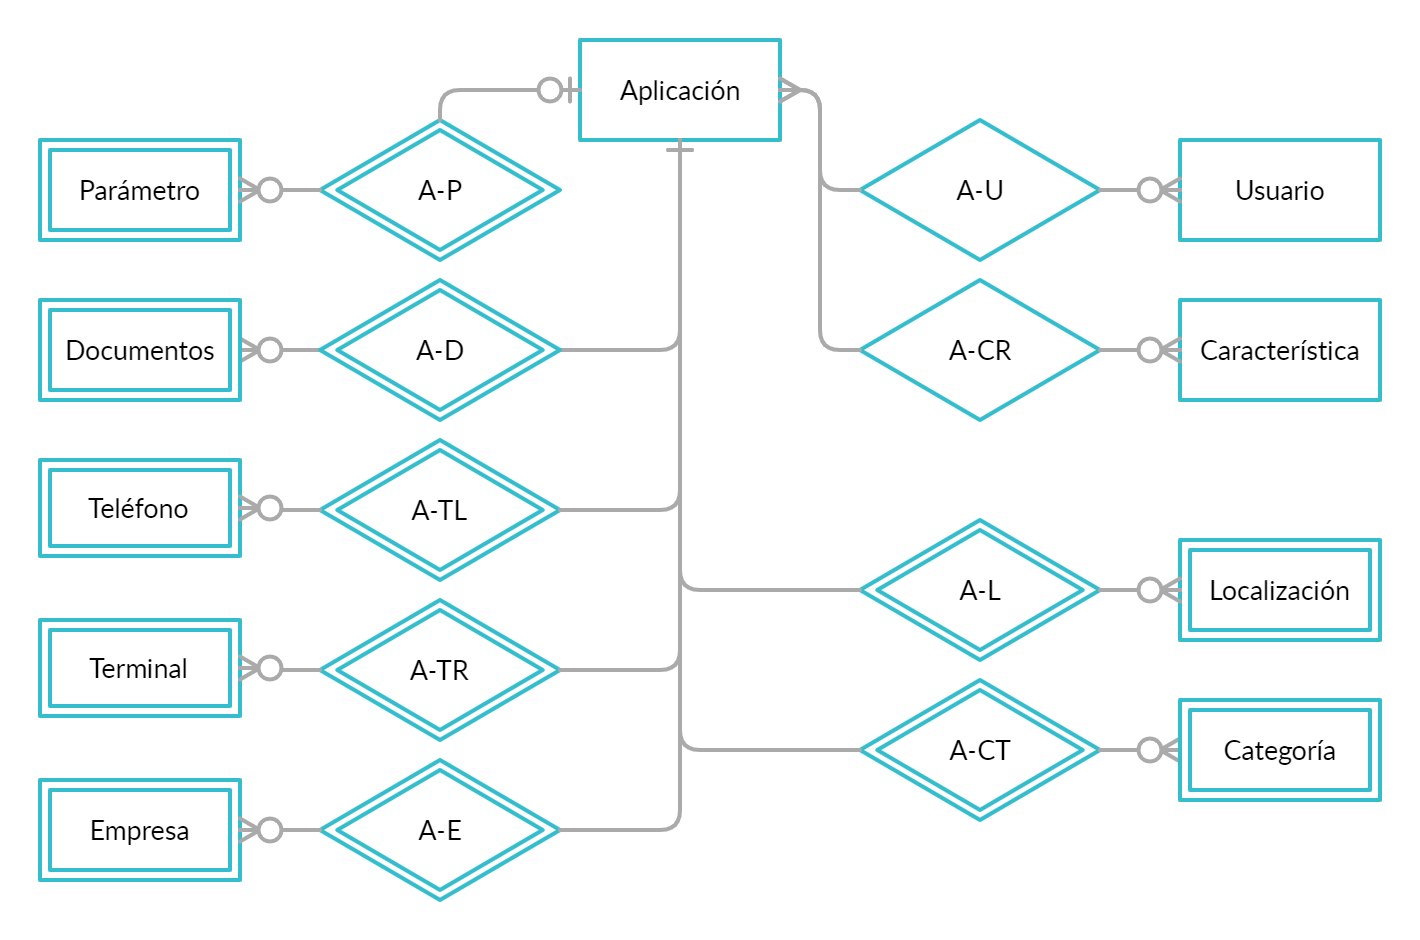
\includegraphics[scale=.31]{PushNews E-R 1}
    \caption{Aplicación como entidad fuerte}
    \label{fig:diagram-entidad-interrelacion-1}
\end{figure}

\begin{figure}[h]
    \centering
    % https://app.creately.com/diagram/FGzbpRaBqk7/edit
    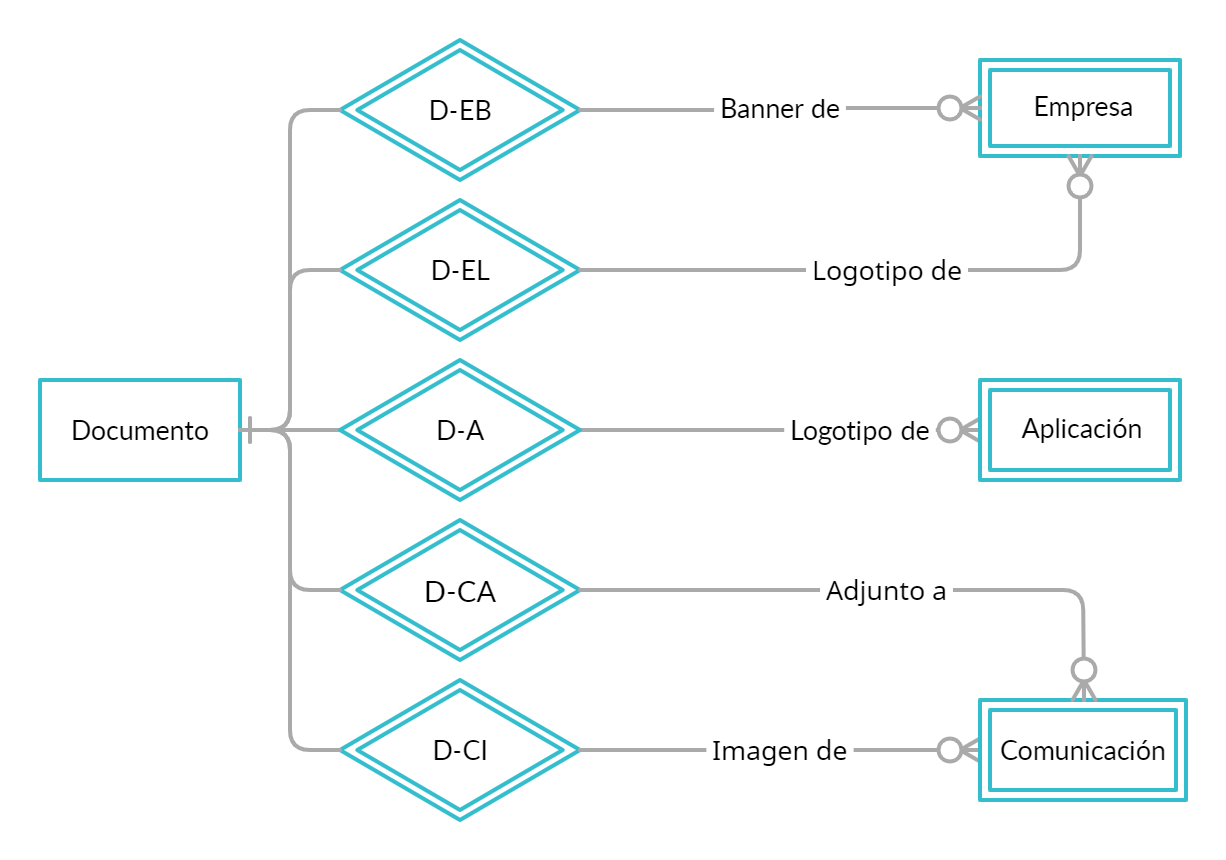
\includegraphics[scale=.31]{PushNews E-R 2}
    \caption{Documento como entidad fuerte}
    \label{fig:diagram-entidad-interrelacion-2}
\end{figure}

\begin{figure}[h]
    \centering
    % https://app.creately.com/diagram/rUhAbYQdpj2/edit
    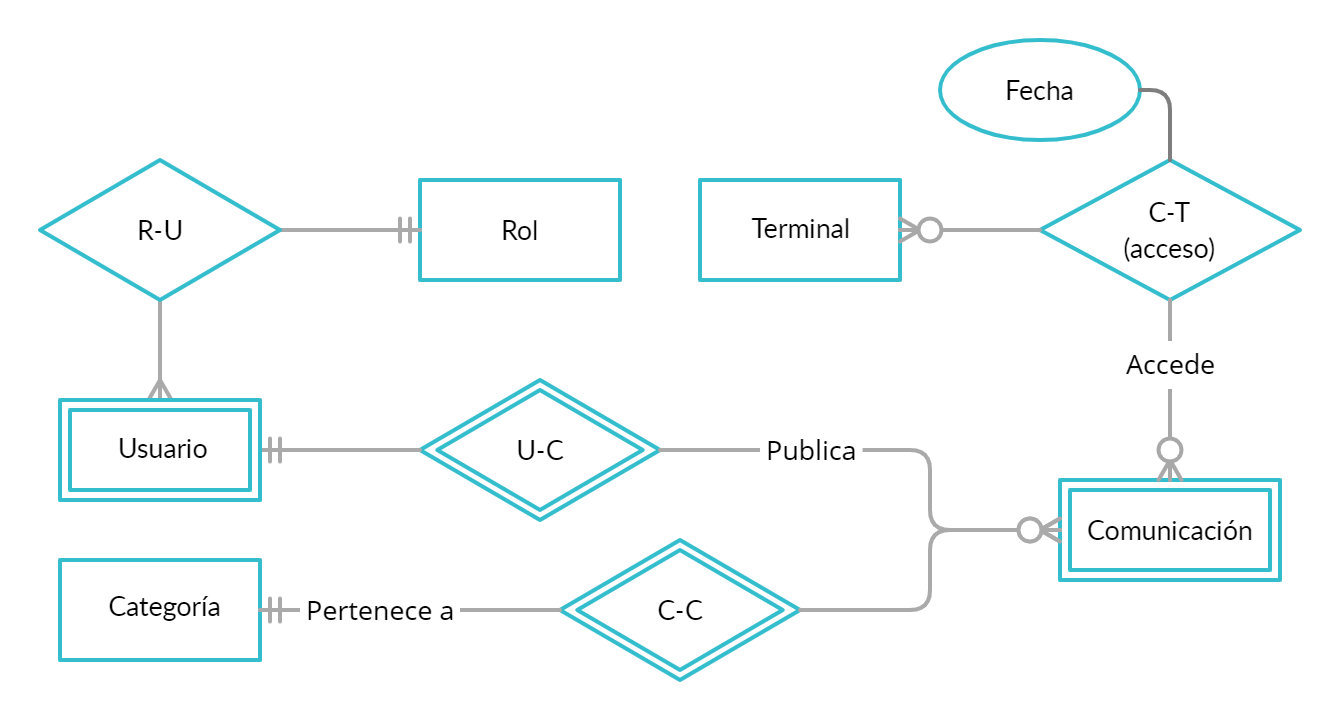
\includegraphics[scale=.31]{PushNews E-R 3}
    \caption{Resto de relaciones}
    \label{fig:diagram-entidad-interrelacion-2}
\end{figure}
\chapter{Análisis funcional}
En este capítulo se detalla el funcionamiento del sistema. Primero se identificará a los actores que intervienen en el sistema, indicando los objetivos de cada uno. A continuación se presentarán los escenarios empleando casos de uso. Por último se detallarán las interacciones entre los actores y los demás elementos del sistema en los principales escenarios mediante diagramas de secuencia.

%%%%%%%%%%%%%%%%%%%%%%%%%%%%%%%%%%%%%%%%%%%%%%%%%%%%%%%%%%%%%%%%%%%%%%%%%%%%%%%%%%%%%%%%%%%%%%%%%%%
%%%%%%%%%%%%%%%%%%%%%%%%%%%%%%%%%%%%%%%%%%%%%%%%%%%%%%%%%%%%%%%%%%%%%%%%%%%%%%%%%%%%%%%%%%%%%%%%%%%
%%%%%%%%%%%%%%%%%%%%%%%%%%%%%%%%%%%%%%%%%%%%%%%%%%%%%%%%%%%%%%%%%%%%%%%%%%%%%%%%%%%%%%%%%%%%%%%%%%%
%%%%%%%%%%%%%%%%%%%%%%%%%%%%%%%%%%%%%%%%%%%%%%%%%%%%%%%%%%%%%%%%%%%%%%%%%%%%%%%%%%%%%%%%%%%%%%%%%%%
%%%%%%%%%%%%%%%%%%%%%%%%%%%%%%%%%%%%%%%%%%%%%%%%%%%%%%%%%%%%%%%%%%%%%%%%%%%%%%%%%%%%%%%%%%%%%%%%%%%
\section{Identificación de actores}
Como ya se introdujo en \ref{objetivos-especificos-gestor-contenidos}, en \emph{PushNews} existen tres tipos de actores o tres perfiles. A continuación se profundizará en los objetivos de cada uno de ellos.

\subsection{Lector}
Cualquier usuario que, incluso sin estar previamente registrado y sin haberse identificado en el sistema, consulte una comunicación. Los principales objetivos de los lectores son:
\begin{enumerate}
    \item Visualizar las comunicaciones publicadas.
    \item Obtener los recursos adjuntos a las comunicaciones (imágenes, documentos\dots).
    \item Saber cuando una nueva comunicación es publicada.
\end{enumerate}

\subsection{Editor}
Generalmente, los editores pertenecerán a la organizaciones de los clientes y su misión es publicar y mantener las comunicaciones así como consultar las métricas. Sus objetivos más importantes son:
\begin{enumerate}
    \item Publicar comunicaciones
    \item Gestión o mantenimiento de las comunicaciones (modificación, eliminación\dots)
    \item Gestión de las categorías de comunicaciones de la aplicación.
    \item Gestión de otros datos de las aplicaciones como lugares de interés, teléfonos, etc.
    \item Ver las métricas de accesos a las comunicaciones
\end{enumerate}

\subsection{Administrador}
Los administradores se encargan del mantenimiento del sistema desde la organización de \emph{PushNews}. Entre sus objetivos principales encontramos:
\begin{enumerate}
    \item Mantenimiento general del servicio.
    \item Administrar las aplicaciones (altas, bajas, etc\dots).
    \item Administrar las características asociadas a las aplicaciones.
    \item Administración de los usuarios (editores) de las aplicaciones. 
    \item Realizar labores de editor de cualquier aplicación.
\end{enumerate}

%%%%%%%%%%%%%%%%%%%%%%%%%%%%%%%%%%%%%%%%%%%%%%%%%%%%%%%%%%%%%%%%%%%%%%%%%%%%%%%%%%%%%%%%%%%%%%%%%%%
%%%%%%%%%%%%%%%%%%%%%%%%%%%%%%%%%%%%%%%%%%%%%%%%%%%%%%%%%%%%%%%%%%%%%%%%%%%%%%%%%%%%%%%%%%%%%%%%%%%
%%%%%%%%%%%%%%%%%%%%%%%%%%%%%%%%%%%%%%%%%%%%%%%%%%%%%%%%%%%%%%%%%%%%%%%%%%%%%%%%%%%%%%%%%%%%%%%%%%%
%%%%%%%%%%%%%%%%%%%%%%%%%%%%%%%%%%%%%%%%%%%%%%%%%%%%%%%%%%%%%%%%%%%%%%%%%%%%%%%%%%%%%%%%%%%%%%%%%%%
%%%%%%%%%%%%%%%%%%%%%%%%%%%%%%%%%%%%%%%%%%%%%%%%%%%%%%%%%%%%%%%%%%%%%%%%%%%%%%%%%%%%%%%%%%%%%%%%%%%
\section{Análisis de casos de uso}
Según Larman, un caso de uso es ``una colección de escenarios con éxito y fallo relacionados, que describe a los actores utilizando un sistema para satisfacer un objetivo.'' \cite{Larman2004}. En este apartado se detallarán los principales casos de uso del sistema.

%%%%%%%%%%%%%%%%%%%%%%%%%%%%%%%%%%%%%%%%%%%%%%%%%%%%%%%%%%%%%%%%%%%%%%%%%%%%%%%%%%%%%%%%%%%%%%%%%%%
%%%%%%%%%%%%%%%%%%%%%%%%%%%%%%%%%%%%%%%%%%%%%%%%%%%%%%%%%%%%%%%%%%%%%%%%%%%%%%%%%%%%%%%%%%%%%%%%%%%
%%%%%%%%%%%%%%%%%%%%%%%%%%%%%%%%%%%%%%%%%%%%%%%%%%%%%%%%%%%%%%%%%%%%%%%%%%%%%%%%%%%%%%%%%%%%%%%%%%%
%%%%%%%%%%%%%%%%%%%%%%%%%%%%%%%%%%%%%%%%%%%%%%%%%%%%%%%%%%%%%%%%%%%%%%%%%%%%%%%%%%%%%%%%%%%%%%%%%%%
%%%%%%%%%%%%%%%%%%%%%%%%%%%%%%%%%%%%%%%%%%%%%%%%%%%%%%%%%%%%%%%%%%%%%%%%%%%%%%%%%%%%%%%%%%%%%%%%%%%
\section{Diagramas de secuencia}
\part{Diseño}
\include{capitulos/301-diseño-de-datos}
\include{capitulos/302-diseño-de-clases}
\chapter{Arquitectura}

\section{Patrón MVC}

Modelo-vista-controlador (MVC) es un patrón de arquitectura de software que separa los datos y principalmente lo que es la lógica de negocio de una aplicación de su representación y el módulo encargado de gestionar los eventos y las comunicaciones. Para ello MVC propone la construcción de tres componentes distintos que son el modelo, la vista y el controlador, es decir, por un lado define componentes para la representación de la información, y por otro lado para la interacción del usuario. Este patrón de arquitectura de software se basa en las ideas de reutilización de código y la separación de conceptos, características que buscan facilitar la tarea de desarrollo de aplicaciones y su posterior mantenimiento \cite{wiki-mvc}.

\begin{figure}[h]
    \centering
    \begin{tikzpicture}[node distance=1cm, auto]
        \tikzset{
            mynode/.style={rectangle,rounded corners,draw=black, top color=white, bottom color=yellow!50,very thick, inner sep=1em, minimum size=3em, text centered},
            myarrow/.style={->, >=latex', shorten >=1pt, thick},
            mylabel/.style={text width=7em, text centered} 
        }
        \node[mynode] (controlador) {Controlador};
        \node[below=3cm of controlador] (dummy) {}; 
        \node[mynode, left=of dummy] (vista) {Vista};
        \node[mynode, right=of dummy] (modelo) {Modelo};
        
        \draw[myarrow] (controlador.south) -- (modelo.north);	
        \draw[myarrow] (vista.north) -- (controlador.south);
        \draw[myarrow] (modelo.west) -- (vista.east);
    \end{tikzpicture}
    \medskip
    \caption{Esquema de la arquitectura Modelo-Vista-Controlador}
\end{figure}

\section{Artefactos}

\begin{figure}[ht]
    \centering
    \begin{tikzpicture}[every fit/.style={inner sep=0pt, outer sep=0pt, draw}]
      \begin{scope}
        \node [fit={( 0,0) (12,1)}, label=center:{Acceso a datos}] {};
        \node [fit={( 0,1) (12,2)}, label=center:{Biblioteca de Negocio}] {};
        \node [fit={( 0,2) ( 4,3)}, label=center:{Aplicación WEB}] {};
        \node [fit={( 4,2) ( 9,3)}, label=center:{Servicio WEB}] {};
        \node [fit={( 9,2) (12,3)}, label=center:{Pr. Auxiliares}] {};
        \node [fit={( 4,3) ( 6,4)}, label=center:{App 1}] {};
        \node [fit={( 6,3) ( 7,4)}, label=center:{\dots}] {};
        \node [fit={( 7,3) ( 9,4)}, label=center:{App N}] {};
      \end{scope}
    \end{tikzpicture}
  \end{figure}
\chapter{Bibliotecas de negocio}

Soportan la lógica de negocio, el esquema de autenticación y autorización y el acceso a datos. Enfoque por tipo de entidad.

\section{Biblioteca de persistencia}


\section{Operaciones de negocio}
\chapter{Aplicación WEB}
La parte WEB de este proyecto  --incluído el servicio para las apps-- estará construida con .NET MVC, un framework de Microsoft para el desarrollo de aplicaciones WEB que implementa el patrón de diseño modelo-vista-controlador. .NET MVC es software libre y se distribuye bajo licencia Apache 2.0.

\section{Áreas}

\section{Filtros de acción}

\section{Controladores}

\section{Modelos}

\section{Vistas}

\section{Servicios}
\subsection{Seguridad y autenticación}
Windows Identity Foundation
\subsection{Servicio de correo electrónico}
\subsection{Mensajería push}
\chapter{Servicio web}
\chapter{Programas auxiliares}
\chapter{Aplicación móvil tipo}
\include{capitulos/309-diseño-de-la-interfaz}
\part{Pruebas}
\part{Conclusiones y futuras mejoras}
\chapter{Conclusiones}
\chapter{Futuras mejoras}

\section{Capa de servicios}
Exponer clases POCO a modo de vistas en lugar de exponer las entidades. Es decir, PersonasServicio.BuscarPersona() debe devolver PersonaModel y no PersonaEntity.

\section{Aplicación web}

\subsection{Backend}
Inyección de dependencias
Prescindir de OWIN

\subsection{Frontend}
Sustituir Telerik por otro Framework

\subsection{Nuevos módulos de características}

\subsection{Explorador de documentos de la aplicación}
Componente para gestionar y reutilizar documentos asociados a la aplicación.
\cleardoublepage

% BIBLIOGRAFÍA -----------------------------------------------------------------
\bibliographystyle{ieeetr}
\renewcommand{\refname}{Bibliografía}
\bibliography{00-memoria-tecnica}
\addcontentsline{toc}{part}{Bibliografía}
\clearpage
% ------------------------------------------------------------------------------

\end{document}